\chapter{Chemistry}

\noindent
\textbf{Everything there is to know about chemistry} -- excerpted from ``Everything you need to know about school'' in the September 16, 2008 edition of the Seattle periodical \textit{The Stranger}:

\vskip 10pt {\narrower \noindent \baselineskip5pt

Stuff is made up of different arrangements of atoms; atoms are made up of nucleus surrounded by buzzing electrons.  The outer shell always wants to be filled with eight electrons.  So, any arrangement that gets you there -- sodium with chloride, oxygen with two hydrogens, carbon with four chlorides -- will work.  This is why the periodic table has eight columns and helium (with eight outer electrons of its own) doesn't explode.  Some arrangements adding up to eight shared electrons are happier than others.  Chemical reactions rearrange from less stable to more stable arrangements on their own, giving off energy in the process.  To make a less stable arrangement, you have to put in energy as payment.  Chemistry is simply accounting: You must not gain or lose atoms at any point.  Ignore the nuclear physicists at this point.

\par} \vskip 10pt

As suggested by this quote, chemistry is the study of matter (stuff) on an atomic scale.  It is relevant to industrial instrumentation because so many industrial processes rely on specific chemical reactions to achieve desired outcomes, and we must use instruments to monitor and regulate these chemical reactions.  Chemistry can be a confounding subject of study, principally because it seems to defy any simple rule.  Many of the ``rules'' learned by chemistry students, such as the rule of eight electrons referenced in the humorous quote, are not general and in fact only apply to certain elements in the Periodic Table.  It should be noted that helium is actually an exception to this rule (an atom of helium only has two electrons, not eight -- but at least the quote was correct in saying helium doesn't explode!).  It should also be noted that only a small portion of the Periodic Table has eight columns -- most of the table in fact has \textit{eighteen} columns.

Perhaps the most accurate portion of the quote is where it tells us atoms are never lost or gained in a chemical reaction: every atom entering a reaction must somewhere exit that reaction.  This simple rule goes by the clumsy name of \textit{stoichiometry} and it is inviolable for all practical purposes.  Chemistry, therefore, is the shuffling of atoms between different arrangements which we call \textit{molecules}.



\filbreak

Chemistry is the study of matter: in particular how and why atoms join with one another to form molecules, and the processes by which molecules may be formed and re-formed.  Any process where atoms either join with one another to form molecules, or break apart to become individual atoms, is called a \textit{chemical reaction}.  Applications of chemistry abound, from the formation of rocks and minerals in the Earth to industrial processes to the processes of organic life itself.  Chemistry plays a particularly important role in industrial instrumentation in the form of devices called \textit{analyzers} which exist to measure concentrations of certain chemicals.  Analytical instrumentation is essential for industrial processes such as wastewater treatment, combustion, and fermentation to proceed safely and efficiently.  Analyzers are also essential for quantitatively tracking pollutants emitted by industrial processes.

Like so many other areas of physical science, the patterns and limits we see in chemical reactions are dominated by two fundamental laws of physics: the \textit{Conservation of Mass} and the \textit{Conservation of Energy}.  The particles of matter comprising atoms have the ability to store energy in potential form, and their tendency is to ``seek'' states having the lowest available energy\footnote{This generally means to seek the \textit{lowest} gross potential energy, but there are important exceptions where chemical reactions actually proceed in the opposite direction (with atoms seeking \textit{higher} energy states and absorbing energy from the surrounding environment to achieve those higher states).  A more general and consistent understanding of matter and energy interactions involves a more complex concept called \textit{entropy}, and a related concept known as \textit{Gibbs Free Energy}.}.  The arrangement of electrons around the nucleus of an atom is largely dictated by the tendency of electrons to ``prefer'' stable energy states, and so is the formation of molecules (atoms bonded together): electrons seeking energy states least liable to disturbance.  The rest, as they say, is mere detail.  \index{Chemistry}  \index{Conservation of Mass}  \index{Conservation of Energy}  \index{Entropy}  \index{Gibbs free energy}

\vskip 10pt

We exploit this property of energy storage in the fuels we use.  Atoms bound together to form molecules are in a lower energy state than when they exist as separate atoms.  Therefore, an investment of energy is required to force molecules apart (into separate atoms), and energy is returned (released) when atoms join together to form molecules.  The combustion of a \textit{fuel}, for example, is nothing more than a process of the atoms in relatively unstable (high-energy) fuel molecules joining with oxygen atoms in air to form stable (low-energy) molecules such as water (H$_{2}$O) and carbon dioxide (CO$_{2}$).

Natural gas, for example, is a relatively stable combination of hydrogen (H) and carbon (C) atoms, mostly in the form of molecules with a 4:1 hydrogen-to-carbon ratio (CH$_{4}$).  However, when placed in the vicinity of free oxygen (O) atoms, and given enough energy (a spark) to cause the hydrogen and carbon atoms to separate from each other, the hydrogen atoms strongly bond with oxygen atoms to form water molecules (H$_{2}$O), while the carbon atoms also strongly bond with oxygen atoms to form carbon dioxide molecules (CO$_{2}$).  These strong bonds formed between hydrogen, carbon, and oxygen in the water and carbon dioxide molecules are the result of electrons within those atoms seeking lower energy states than they possessed while forming molecules of natural gas (CH$_{4}$).  In other words, the electrons binding hydrogen and carbon atoms together to form natural gas are at higher energy states than the electrons binding hydrogen and carbon atoms to oxygen atoms to form water and carbon dioxide, respectively.  As those electrons attain lower energy states, they difference of energy must go somewhere (since energy cannot be created or destroyed), and so the chemical reaction releases that energy in the forms of heat and light.  This is what you see and feel in the presence of a natural gas flame: the heat and light emitted by hydrogen and carbon atoms joining with oxygen atoms.

\vskip 10pt

The Law of Mass Conservation plays an important role in chemistry as well.  When atoms join to form molecules, their masses add.  That is, the mass of a molecule is precisely equal\footnote{This statement is not perfectly honest.  When atoms join to form molecules, the subsequent release of energy is translated into an incredibly small loss of mass for the molecule, as described by Albert Einstein's famous mass-energy equation $E = mc^2$.  However, this mass discrepancy is so small (typically less than one part per \textit{billion} of the original mass!), we may safely ignore it for the purposes of understanding chemical reactions in industrial processes.  This is what the humorous quote at the start of this chapter meant when it said ``ignore the nuclear physicists at this point''.} to the mass of its constituent atoms.  Furthermore, the total mass is unaffected when atoms separate and then re-join to form different molecules.  In our natural gas combustion example, the mass of the CH$_{4}$ molecules plus the mass of the oxygen atoms they combust with precisely equals the sum total mass of the water and carbon dioxide molecules produced by the combustion.  Another way of saying this is that all mass entering a chemical reaction must equal the mass exiting that same reaction.  Chemical engineers apply this principle when they calculate \textit{mass balance} in a chemical process: accounting for all mass entering and exiting the process based on the safe assumption that no mass will be gained or lost.

\vskip 10pt

Too many other practical applications of chemistry exist to summarize in these pages, but this chapter aims to give you a foundation to understand basic chemistry concepts necessary to comprehend the function of certain instruments (notably \textit{analyzers}) and processes.








\filbreak
\section{Terms and Definitions}

\begin{itemize}
\item \textit{Atom}: the smallest unit of matter that may be isolated by chemical means. \index{Atom}
\item \textit{Particle}: a part of an atom, separable from the other portions only by levels of energy far in excess of chemical reactions. \index{Particle}
\item \textit{Proton}: a type of ``elementary'' particle, found in the nucleus of an atom, possessing a positive electrical charge. \index{Proton}
\item \textit{Neutron}: a type of ``elementary'' particle, found in the nucleus of an atom, possessing no electrical charge, and having nearly the same amount of mass as a proton. \index{Neutron}
\item \textit{Electron}: a type of ``elementary'' particle, found in regions surrounding the nucleus of an atom, possessing a negative electrical charge, and having just a small fraction of the mass of a proton or neutron. \index{Electron}
\item \textit{Element}: a substance composed of atoms all sharing the same number of protons in their nuclei (e.g. hydrogen, helium, nitrogen, iron, cesium, fluorine). \index{Element}
\item \textit{Atomic number}: the number of protons in the nucleus of an atom -- this quantity defines the chemical identity of an atom.  \index{Atomic number}
\item \textit{Atomic mass} or \textit{Atomic weight}: the total number of elementary particles in the nucleus of an atom (protons + neutrons) -- this quantity defines the vast majority of an atom's mass, since the only other elementary particle (electrons) are so light-weight by comparison to protons and neutrons.  \index{Atomic weight}  \index{Atomic mass}
\item \textit{Ion}: an atom or molecule that is not electrically balanced (i.e. equal numbers of protons and electrons). \index{Ion}
\subitem $\rightarrow$ \textit{Cation}: a positively-charged ion, called a ``cation'' because it is attracted toward the negative electrode (cathode) immersed in a fluid solution.  \index{Cation}
\subitem $\rightarrow$ \textit{Anion}: a negatively-charged ion, called an ``anion'' because it is attracted toward the positive electrode (anode) immersed in a fluid solution.  \index{Anion}
\item \textit{Isotope}: a variation on the theme of an element -- atoms sharing the same number of protons in their nuclei, but having different numbers of neutrons, are called ``isotopes'' (e.g. uranium-235 versus uranium-238).  \index{Isotope}
\item \textit{Molecule}: the smallest unit of matter composed of two or more atoms joined by electron interaction in a fixed ratio (e.g. water: H$_{2}$O).  The smallest unit of a \textit{compound}.  \index{Molecule}
\item \textit{Compound}: a substance composed of identical molecules (e.g. pure water). \index{Compound}
\item \textit{Isomer}: a variation on the theme of a compound -- molecules sharing the same numbers and types of atoms, but having different structural forms, are called ``isomers''.  For example, the sugars glucose and fructose are isomers, both having the same formula C$_{6}$H$_{12}$O$_{6}$ but having different molecular structures.  An isomer is to a molecule as an isotope is to an atomic nucleus.  \index{Isomer}
\item \textit{Mixture}: a substance composed of different atoms or molecules not electronically bonded to each other. \index{Mixture}
\item \textit{Solution}: an homogeneous mixture at the molecular level (different atoms/molecules thoroughly mixed together).  A solution may be a gas, a liquid, or a solid (e.g. air, saltwater, steel).    \index{Solution}
\subitem $\rightarrow$ \textit{Solvent}: the majority element or compound in a solution.  Chemists usually consider water to be the \textit{universal solvent}.  \index{Solvent}  \index{Universal solvent}
\subitem $\rightarrow$ \textit{Solute}: the minority element or compound in a solution (may be more than one).  \index{Solute}
\subitem $\rightarrow$ \textit{Precipitate}: (noun) solute that has ``fallen out of solution'' due to the solution being saturated with that element or compound; (verb) the process of solute separating from the rest of the solution.  (e.g. If you mix too much salt with water, some of the salt will \textit{precipitate} out of the water to form a solid pile at the bottom.)  \index{Precipitate}
\subitem $\rightarrow$ \textit{Supernatant}: the solution remaining above the precipitate.  \index{Supernatant}
\item \textit{Suspension}: an heterogeneous mixture where separation occurs due to gravity (e.g. mud).  \index{Suspension}
\item \textit{Colloid} or \textit{Colloidal suspension}: an heterogeneous mixture where separation either does not occur or occurs at a negligible pace under the influence of gravity (e.g. milk).  \index{Colloid}
\subitem $\rightarrow$ \textit{Aerosol}: A colloid formed of a solid or liquid substance dispersed in a gas medium. \index{Aerosol}
\subitem $\rightarrow$ \textit{Foam}: A colloid formed of a gas dispersed in either a liquid or a solid medium. \index{Foam}
\subitem $\rightarrow$ \textit{Emulsion}: A colloid formed of a liquid dispersed in either a liquid or a solid medium. \index{Emulsion}
\subitem $\rightarrow$ \textit{Sol}: A colloid formed of a solid dispersed in either a liquid or a solid medium. \index{Sol}
\end{itemize}






\filbreak
\section{Atomic theory and chemical symbols}

The three ``elementary'' particles of matter comprising all atoms are \textit{electrons}, \textit{protons}, and \textit{neutrons}.  Combinations of these three particle types in various whole-number quantities constitute every type of atom.  These fundamental particles are absolutely miniscule in comparison to the macroscopic existence of human beings.  Just to illustrate, the mass of a single proton is approximately $1.67 \times 10^{-27}$ kilograms: written without scientific notation, it would be 0.00000000000000000000000000167 kg.  An electron is even smaller: weighing in at $9.11 \times 10^{-31}$ kg (about \textit{1800 times} less mass than a proton!).  Being far smaller in size than a wavelength of visible light\footnote{In order for a wave of light to be influenced at all by an object, that object must be at least the size of the wave's length.  To use an analogy with water waves, it would be comparing the interaction of a water wave on a beach against a large rock (a disturbance in the wave pattern) versus the non-disturbance of that same wave as it encounters a small buoy.}, we cannot see these particles even with the most powerful optical microscope.

Protons and neutrons are very tightly bound together in the nucleus (center) of an atom.  This bond is so secure that only extraordinary forces are able to pry an atom's nucleus apart.  Suffice it to say, one cannot disturb the stability of an atomic nucleus by rubbing, cutting, grinding, heating, smashing, or any other macroscopic physical process.  The force binding protons and neutrons together in the nucleus is known as the \textit{strong nuclear force}.  \index{Strong nuclear force}

Electrons ``orbit'' the nucleus of atoms, and are held in proximity to those nuclei by electrostatic attraction (the so-called \textit{electromagnetic force}), which is many orders of magnitude weaker than the strong nuclear force.  Thus, electrons \textit{can} be dislodged from or added to atoms through the action of macroscopic forces such as rubbing, cutting, grinding, heating, etc.  It is the changeable configurations of electrons that accounts for different atoms joining together to form \textit{molecules}.  \index{Electromagnetic force}

The chemical identity of any atom is a simple and direct function of how many protons that atom has in its nucleus.  Each nitrogen atom, for example, has seven (7) protons in its nucleus.  This quantity is called the \textit{atomic number} of an atom.  In order for an atom to have a net neutral electric charge, there must be as many electrons orbiting the nucleus as there are protons in the nucleus, since protons are positively charged and electrons are negatively charged (equal and opposite electric charges, each).  Therefore, a neutral atom of nitrogen will have seven electrons orbiting around the nucleus, electrically balancing the seven protons within the nucleus.  \index{Atomic number}

The number of neutrons within the nucleus of an atom does not affect the atom's chemical identity, but it may affect its nuclear properties (e.g. whether or not it is radioactive; to what degree it captures certain forms of radiation, etc.).  For example, most nitrogen atoms have seven neutrons along with seven protons in their nuclei, giving a total nuclear particle count of fourteen -- the atomic \textit{mass} of the atom, sometimes called the atomic \textit{weight}.  However, it is possible for a nitrogen atom to have eight neutrons (an atomic mass of fifteen) and still be ``nitrogen,'' with all the same chemical properties.  \index{Atomic mass}  \index{Atomic weight}

\filbreak

A tremendously simplified model of a common nitrogen atom is shown here, with 7 protons and 7 neutrons in the nucleus, and 7 electrons in ``orbit'' around the nucleus:

$$\includegraphics{chemistry06.eps}$$

The atomic number of this atom (the number of protons in the nucleus) is seven, which is what defines it as nitrogen.  The \textit{atomic mass} of this atom (the sum of protons and neutrons in the nucleus) is fourteen.  The chemical symbol for this atom is shown here:

$$\includegraphics{chemistry07.eps}$$

The atomic number is redundant to the letter ``N'' for nitrogen, since only the element nitrogen can have an atomic number of seven.  The atomic mass is only relevant when we need to distinguish one \textit{isotope} of nitrogen from another (variations of elements having the same number of protons but different numbers of neutrons), and this is seldom because the chemical properties of isotopes are identical -- only their masses differ.  For these reasons, you will usually find no left-hand subscripts or superscripts placed near chemical symbols of elements in chemical expressions.

\vskip 10pt

\filbreak

By contrast, subscripts and superscripts placed to the right of a chemical symbol have very important meanings in chemistry.  A right-hand subscript refers to the number of atoms bound together to form a molecule.  A right-hand superscript refers to the electrical charge possessed by an atom (or by a molecule) by virtue of the number of electrons not matching the number of protons:

An N$_{2}$ molecule may be represented simplistically as follows, the two nitrogen atoms joined by a mutual sharing of three of its highest-energy (valence) electrons, shown in this illustration as those electrons residing in the largest-diameter ``orbits''.  Incidentally, this ``triple bond'' characterizing the nitrogen molecule is very strong (the more electrons participating in the joining of two atoms, the stronger the bond, all other factors being equal):

$$\includegraphics{chemistry08.eps}$$

An N$^{3-}$ ion is an atom of nitrogen having three more electrons than it normally would when electrically balanced:

$$\includegraphics{chemistry09.eps}$$

\vskip 10pt

\filbreak

A chemical \textit{formula} is a written description of a molecule's constituent atoms.  Ethanol (ethyl alcohol), for example, is a conglomerate of two carbon atoms, six hydrogen atoms, and one oxygen atom.  One way to express this structure is to write the following formula for ethanol, the right-hand subscripts showing the relative quantities of atoms in each ethanol molecule:

$$\hbox{C}_2 \hbox{H}_6 \hbox{O}$$

This is called a \textit{molecular formula}, because it shows the proportions of atom types comprising each molecule.  \index{Molecular chemical formula}

\vskip 10pt

\filbreak

A more common way to write the formula for ethanol, though, is this:

$$\hbox{C}_2 \hbox{H}_5 \hbox{OH}$$

Here, an attempt is made to show the physical structure of the ethanol molecule, where one of the hydrogen atoms is located further away from the others.  This is called a \textit{structural formula}.  If more detail of the bonds between atoms in a molecule is needed, a semi-graphic representation called a \textit{displayed formula} (also known as an \textit{expanded structural formula}) may be used in lieu of a structural formula:  \index{Structural chemical formula}  \index{Displayed chemical formula}  \index{Expanded structural formula}

$$\includegraphics{chemistry11.eps}$$

Each letter in a displayed formula represents a single atom within that molecule, and each line segment in a displayed formula represents a bond between two.

\vskip 10pt

\filbreak

In organic chemistry -- the study of molecules principally centered around \textit{carbon} atoms -- a special type of notation is used to show the structural detail of the molecule with fewer lines and letters than a displayed formula.  This notation is called a \textit{line drawing}, where each line segment represents a single electron bond\footnote{One line represents a single bond, which is one electron shared per bound atom.  Two parallel lines represent a \textit{double bond}, where each carbon atom shares two of its valence electrons with the neighboring atom.  Three parallel lines represent a triple bond, where each atom shares three of its outer electrons with the neighboring atom.} to a carbon atom, each vertex and line-end represents the location of a carbon atom, and any hydrogen atoms directly bound to a carbon atom are simply omitted for simplicity.  Compare and contrast these displayed formulae and line drawings for a few different organic compounds:

$$\includegraphics{chemistry23.eps}$$

An important principle in organic chemistry is that carbon atoms prefer to form exactly \textit{four} bonds with surrounding atoms\footnote{Incidentally, nitrogen atoms preferentially form exactly \textit{three} bonds, and oxygen atoms exactly \textit{two} bonds.  The reason for this pattern is the particular patterns of electrons orbiting each of these atoms, and their respective energy levels.  For more information on this, see section \ref{Electronic structure} beginning on page \pageref{Electronic structure}.}.  This fact is exploited in line-drawing notation where any bonds not explicitly shown at a vertex are assumed to be single-bonds with hydrogen atoms, enough of them to bring the total number of bonds with that carbon atom to four.  Since a great many organic compounds are principally comprised of carbon and hydrogen, the line-drawing symbols for these molecules tend to be more lines than letters.

\vskip 10pt

\filbreak

Chemical engineers often perform mass and energy balance calculations for processes where \textit{mixtures} of similar compounds exist.  Wastewater treatment is one example, where an array of organic compounds must all be treated through oxidation (chemical reaction with oxygen).  In such cases, it is common for chemical engineers to write formulae expressing the \textit{average} ratios of elements, so that they may calculate the quantity of reactant(s) needed to complete the desired chemical reaction with compounds in the mixture.  Primary sludge clarified from municipal wastewater, for example, may be represented by the \textit{compositional formula} C$_{22}$H$_{39}$O$_{10}$N.  This does not suggest the existence of some monstrous molecule consisting of twenty-two carbon atoms, thirty-nine hydrogen atoms, ten oxygen atoms, and a lone nitrogen atom somewhere in a sample of sludge, but rather that the combined \textit{average} carbon, hydrogen, oxygen, and nitrogen quantities in that sludge exist in a variety of molecular forms in these approximate proportions.  This aggregate formula expression helps the engineer quantify the gross chemical characteristics of the sludge, and from that determine how much oxygen will be necessary to completely oxidize it.  \index{Compositional chemical formula}

Sometimes, compositional formulae are written with non-integer subscripts.  An example of this would be the compositional formula C$_{4.8}$H$_{8.4}$O$_{2.2}$, which also happens to be an average composition for municipal wastewater sludge (ignoring nitrogen content).  The same formula could just as well have been written C$_{48}$H$_{84}$O$_{22}$, or even C$_{24}$H$_{42}$O$_{11}$, because these subscript values all express the exact same proportions.








\filbreak
\section{Periodic table of the elements}

All substances are comprised of various elements in various combinations and proportions.  Elements may thus be thought of as the building-blocks of matter.  A Periodic Table of the Elements is a table listing the known elements in order of their atomic numbers.  \index{Periodic Table of the Elements}

%\begin{figure}[h]
$$\includegraphics[width=6in]{000.eps}$$
%$$\includegraphics[angle=-90,width=6in]{periodic_table.eps}$$ 
%\caption{Courtesy of National Institute for Standards and Technology (NIST)}
%\end{figure}

Multiple attributes appear for each element in the table.  Two of these attributes -- atomic number and atomic mass -- are directly related to the number of particles in the nucleus of each atom.  We will examine the table's entry for the element \textit{potassium} (K) to explore these concepts.

%$$
\includegraphics{001.eps}$$

Potassium has an \textit{atomic number} (number of protons in the nucleus of each potassium atom) of 19.  This number defines the element.  If we were somehow to add or subtract protons from the nucleus of a potassium atom\footnote{The amount of energy required to rearrange particles in the nucleus for even just a single atom is \textit{tremendous}, lying well outside the energy ranges of chemical reactions.  Such energy levels are the exclusive domain of \textit{nuclear} reactions and high-energy radiation (subatomic particles traveling at high velocity).  The extremely large energy ``investment'' required to alter an atom's nucleus is why atomic identities are so stable.  This is precisely why alchemists of antiquity utterly failed to turn lead into gold: no materials, processes, or techniques they had at their disposal were capable of the targeted energy necessary to dislodge three protons from a nucleus of lead ($_{82}$Pb) to that it would turn into a nucleus of gold ($_{79}$Au).  That, and the fact the alchemists had no clue about atomic structure to begin with, made their endeavor fruitless.}, it would cease being potassium and \textit{transmutate} into a different element.  Note how \textit{every} element in the table has its own unique atomic number, and how each of these numbers is whole (no fractions or decimals).  \index{Atomic number}

The \textit{atomic mass} or \textit{atomic weight} shown for potassium is 39.0983.  This quantity is the sum of protons and neutrons found in the nucleus of each potassium atom.  Like the atomic number (19), we would logically expect the atomic mass to be a whole number as well, since protons and neutrons only come in whole quantities.  The primary reason we see a non-whole number for potassium's atomic mass is that this table reflects the \textit{average} atomic mass of potassium atoms as found in nature.  Some potassium atoms have atomic masses greater than 39, and some have atomic masses less than 39.  We know that the number of protons in every potassium atom is fixed (which is what gives potassium its elemental identity), which means the only quantity that may cause the atomic mass to vary is the number of \textit{neutrons} in the nucleus.  The most common form of potassium ($^{39}$K) atom possesses 19 protons and 20 neutrons in its nucleus, giving it an atomic mass of 39 (19 + 20).  The next most common form of potassium found on Earth is ($^{41}$K), possessing 19 protons and 22 neutrons.   \index{Atomic mass}  \index{Atomic weight} 

We refer to atoms of the same element with differing atomic masses as \textit{isotopes}.  From a chemical perspective, isotopes are identical.  That is to say, they engage in the exact same chemical reactions in the exact same manner.  To use potassium as an example, an atom of $^{39}$K will join with a chlorine atom (Cl) to form the compound \textit{potassium chloride} (KCl) just as readily as an atom of $^{41}$K will join with a chlorine atom to form the same compound.  The three isotopes of hydrogen ($^{1}$H, $^{2}$H, and $^{3}$H: hydrogen, deuterium, and tritium, respectively) are all chemically identical: all are highly flammable, combining with oxygen to create water (H$_{2}$O).  However, deuterium ($^{2}$H) has twice the density of normal hydrogen ($^{1}$H), while tritium ($^{3}$H) has three times the density of normal hydrogen and is highly radioactive!  Isotopes only differ in their mass and in their nuclear properties (such as \textit{radioactivity}: the tendency for a nucleus to spontaneously decay, usually resulting in a loss or gain of protons that subsequently alters the identity of the decayed atom).  \index{Isotopes} \index{Radioactivity}

\vskip 10pt

The Periodic Table is called ``periodic'' because its configuration reveals a repeating pattern of chemical behaviors approximately following atomic number.  Horizontal rows in the table are called \textit{periods}, while vertical columns are called \textit{groups}.  Elements in the same group (vertical column) share similar chemical reactivities -- that is, they tend to engage in the same types of chemical reactions -- despite having different masses and physical properties such as melting point, boiling point, etc.  This \textit{periodicity} is a function of how electrons are arranged around the nucleus of each atom, a subject we will explore in more detail later in this chapter.  As mentioned previously, chemistry is the study of how atoms bond together to form molecules, and this bonding takes place through the interaction of the electrons surrounding the atoms' nuclei.  It makes perfect sense, then, that the configuration of those electrons determine the chemical (bonding) properties of atoms.

\filbreak

Some periodic tables show the \textit{first ionization energy} value for each element -- the amount of energy required to force the first electron of an electrically balanced atom to separate from that atom -- in addition to other attributes such as atomic number and atomic mass.  If we note the ionization energies of the elements, reading each element in turn from left-to-right, starting with period 1 (hydrogen and helium) and progressing to subsequent periods, we see an interesting pattern:

% No blank lines allowed between lines of an \halign structure!
% I use comments (%) instead, so that TeX doesn't choke.

$$\vbox{\offinterlineskip
\halign{\strut
\vrule \quad\hfil # \ \hfil & 
\vrule \quad\hfil # \ \hfil & 
\vrule \quad\hfil # \ \hfil \vrule \cr
\noalign{\hrule}
%
% First row
\textbf{Element} & \textbf{Period} & \textbf{First ionization energy} \cr
 &  & (measured in ``electron-volts'') \cr
%
\noalign{\hrule}
%
% Another row
Hydrogen (H) & 1 & 13.5984 \cr
%
\noalign{\hrule}
%
% Another row
Helium (He) & 1 & 24.5874 \cr
%
\noalign{\hrule}
%
% Another row
Lithium (Li) & 2 & 5.3917 \cr
%
\noalign{\hrule}
%
% Another row
Beryllium (Be) & 2 & 9.3227 \cr
%
\noalign{\hrule}
%
% Another row
Boron (B) & 2 & 8.2980 \cr
%
\noalign{\hrule}
%
% Another row
Carbon (C) & 2 & 11.2603 \cr
%
\noalign{\hrule}
%
% Another row
Nitrogen (N) & 2 & 14.5341 \cr
%
\noalign{\hrule}
%
% Another row
Oxygen (O) & 2 & 13.6181 \cr
%
\noalign{\hrule}
%
% Another row
Fluorine (F) & 2 & 17.4228 \cr
%
\noalign{\hrule}
%
% Another row
Neon (Ne) & 2 & 21.5645 \cr
%
\noalign{\hrule}
%
% Another row
Sodium (Na) & 3 & 5.1391 \cr
%
\noalign{\hrule}
%
% Another row
Magnesium (Mg) & 3 & 7.6462 \cr
%
\noalign{\hrule}
%
% Another row
Aluminum (Al) & 3 & 5.9858 \cr
%
\noalign{\hrule}
%
% Another row
Silicon (Si) & 3 & 8.1517 \cr
%
\noalign{\hrule}
%
% Another row
Phosphorus (P) & 3 & 10.4867 \cr
%
\noalign{\hrule}
%
% Another row
Sulfur (S) & 3 & 10.3600 \cr
%
\noalign{\hrule}
%
% Another row
Chlorine (Cl) & 3 & 12.9676 \cr
%
\noalign{\hrule}
%
% Another row
Argon (Ar) & 3 & 15.7596 \cr
%
\noalign{\hrule}
%
% Another row
Potassium (K) & 4 & 4.3407 \cr
%
\noalign{\hrule}
} % End of \halign 
}$$ % End of \vbox

First ionization energy represents the relative stability of the last electron balancing the electrical charge of an atom.  We see from this table that 24.5874 electron-volts of energy is needed to remove one electron from an electrically-balanced atom of helium (changing He into He$^{1+}$), while only 13.5984 electron-volts of energy is required to do the same to an atom of hydrogen.  This tells us the electron configuration of helium is at a lower energy (and therefore more stable) than that of hydrogen.

\filbreak

The ionization energies increase with increasing atomic number (with an occasional down-step) until the last column of the period is reached, and then there is a comparatively enormous down-step in energy at the first column of a new period.  This pattern is clearly evident when the first ionization energies are plotted against atomic number:

$$\includegraphics{chemistry13.eps}$$

This periodicity suggests that as atoms grow in atomic number, the additional electrons do not simply pile on in random fashion or in a plain and simple progression from inner orbits to outer orbits.  Rather, they ``fill in'' a structured energy pattern, with major changes in structure at the start of each new period.  More details of this structured pattern will be explored later in this chapter.  

The low ionization energy values for all the ``Group 1'' elements (far left-hand column) suggest they are relatively easy to positively ionize, and indeed we find this to be the case through experimentation.  Hydrogen, lithium, sodium, potassium, and the rest all readily become positively-charged ions upon interaction with other atoms, since their low ionization energy values means they may easily lose an electron.

The high ionization energy values for all the ``Group 18'' elements (far right-hand column) suggest they possess a very stable electron structure, which is also verified by experiment.  These are the \textit{noble} elements, possessing very little reactive potential\footnote{It used to be believed that these elements were completely \textit{inert}: incapable of forming molecular bonds with other atoms.  However, this is not precisely true, as some compounds are now known to integrate noble elements.}.  

Looking at the ``Group 17'' column, just to the left of the noble elements, we notice that they are all just one electron shy of the stable electron structure enjoyed by the noble atoms when in their electrically-balanced states.  This suggests it might be easy to \textit{add} one more electron to atoms of these elements, which (once again!) is a principle validated by experiment.  Fluorine, chlorine, bromine, iodine, and even astatine\footnote{All isotopes of astatine (At) are radioactive with very short half-lives, making this element difficult to isolate and study.} all readily ionize negatively, readily accepting an extra electron from surrounding atoms.  As one might expect from this tendency, these elements readily bond through electrostatic attraction with the ``Group 1'' elements (hydrogen, lithium, sodium, potassium, etc.), each ``Group 17'' atom accepting an extra electron from each ``Group 1'' atom which readily provides it.  Ordinary table salt (sodium chloride, or NaCl) is an example of a compound formed by this sort of bond.

Thus, Group 1 and Group 17 elements are both highly reactive in a chemical sense, but in different ways.  Group 1 elements easily form bonds with Group 17 elements, but Group 1 elements do not generally bond (solely) with other Group 1 elements, and likewise Group 17 elements do not generally bond (solely) with other Group 17 elements.  It is the structure of the electrons surrounding each atom's nucleus that determines how those atoms will bond with other atoms.







\filbreak
\section{Electronic structure}

\label{Electronic structure}

Earlier in this chapter you were shown a model of a nitrogen atom with a dense nucleus (comprised of protons and neutrons) surrounded by electrons whirling around like satellites around a planet.  While there are some useful features of this model, it is largely in error.  A more realistic view of atomic structure begins with the realization that electrons do not exist as discrete particles, but rather as wave packets.  In a sense, they orbit the nucleus within certain \textit{areas of probability}, as described by the principles of quantum mechanics.  One way to envision this is to think of an electron's placement around the nucleus in the same way you might picture a city shrouded by a layer of fog.  The electron does not have a discrete location (even though there \textit{is} a discrete number of them found in every atom), but rather may be found anywhere within a certain region to varying degrees of probability.

Things get even stranger the more electrons there are in an atom.  No two electrons may share the same quantum states in the same atom -- a principle called the \textit{Pauli Exclusion Principle}.  This means the electrons surrounding a nucleus must exist in distinct patterns.  Just a few of these patterns are shown here as \textit{orbitals} (regions of high probability where up to two electrons may be found surrounding a nucleus):\footnote{These orbitals just happen to be the 1s, 2p, 3d, and 4f orbitals, as viewed from left to right.  In each case, the nucleus lies at the geometric center of each shape.  In a real atom, all orbitals share the same center, which means any atom having more than two electrons (that's all elements except for hydrogen and helium!) will have multiple orbitals around one nucleus.  This four-set of orbital visualizations shows what some orbitals would look like if viewed in isolation.}  \index{Pauli Exclusion Principle}  \index{Orbital, electron}  \index{Electron orbital}

$$\includegraphics[width=2.5in]{chemistry04.eps}$$

Electrons situate themselves around the nucleus of any atom according to one basic rule: the minimization of potential energy.  That is, the electrons seek the lowest-energy positions available around the nucleus.  Given the electrostatic attraction between negative electrons and the positive nucleus of an atom, there is potential energy stored in the ``elevation'' between an orbiting electron and the nucleus, just as there is gravitational potential energy in any object orbiting a planet.  Electrons lose energy as they situate themselves closer to the nucleus, and it requires an external input of energy to move an electron farther away from its parent nucleus.

In a sense, most of chemistry may be explained by this principle of minimized potential energy.  Electrons ``want'' to ``fall'' as close as they can to the positively-charged nucleus.  However, there is limited ``seating'' around the nucleus.  As described by Pauli's Exclusion Principle, electrons cannot simply pile on top of each other in their quest for minimum energy, but rather must occupy certain regions of space allowed by their unique quantum states.

An analogy\footnote{Please understand that like all analogies, this one merely illustrates a complex concept in terms that are easier to recognize.  Analogies do not \textit{explain} why things work, but merely liken an abstract phenomenon to something more accessible to common experience.} for visualizing this is to picture an atom as if it were an amphitheater, with the stage being the nucleus and the concentric array of seats being places where electrons may reside.  All spectators (electrons) desire to be as close to the stage (nucleus) in an amphitheater (atom) as possible, but since everyone cannot occupy the best seat, people are forced to choose seats at different positions around the stage.  As a result, the inner seats fill first, with most empty seats being furthest away from the stage.  The concept of energy fits neatly into this analogy as well: just as electrons give up \textit{energy} to ``fall into'' lower-energy regions around the nucleus, people must give up \textit{money} to purchase seats closest to the action on stage.

The energy levels available for orbiting electrons are divided into categories of \textit{shells} and \textit{subshells}.  A ``shell'' (or, \textit{principal quantum number}, $n$) describes the main energy level of an electron.  In our amphitheater analogy, this is equivalent to a \textit{tier} or \textit{seating level}.  A ``subshell'' (or, \textit{subsidiary quantum number}, $l$) further divides the energy levels within each electron shell, and assigns different shapes to the electrons' probability ``clouds.''  In the amphitheater analogy, a subshell would be a row of seats within a particular tier.  To make the analogy accurate, we would have to imagine each row of seats in a tier having a different shape (not all arcs or straight lines), with varying degrees of viewing comfort afforded by each shape.  The first row in each tier faces uniformly toward the stage, allowing easy viewing.  Successive rows (subshells) in each tier (shell) contain more seats, but are bent in such a way that the stage is not as easy to view, making these rows less desirable to occupy.  Electron subshells always have an even-numbered electron capacity, analogous to theater rows containing even-numbered quantities of seats, because atomic electrons tend to gather in pairs called \textit{orbitals}.  \index{Shell, electron}  \index{Subshell, electron}  \index{Electron shell}  \index{Orbital, electron}  \index{Electron orbital}

Chemists identify electron shells both by number (the value of the quantum number $n$) and/or by capital letters: the first shell by the letter K, the second by L, the third by M, and the fourth by N.  Higher-order shells exist for atoms requiring\footnote{Truth be told, higher-order shells exist even in simple atoms like hydrogen, but are simply not occupied by that atom's electron(s) unless they are ``excited'' into a higher energy state by an external input of energy.} many electrons (high atomic number), and the lettering pattern is alphabetic (fifth shell is O, sixth is P, etc.).  Each successive shell has a greater number of subshells available, like successive amphitheater tiers having more rows: the low-level tiers closest to the stage having the fewest rows, and the high-level tiers furthest from the stage having the most rows.

A numbering and lettering system is also used by chemists to identify subshells within each shell (the $l$ quantum number value starting with zero, and lower-case letters beginning with ``s''): the first subshell ($l = 0$) in any shell represented by the letter s, the second ($l = 1$) by p, the third ($l = 2$) by d, the fourth ($l = 3$) by f, and all others by successive lower-case letters of the alphabet\footnote{The letters \textit{s}, \textit{p}, \textit{d}, and \textit{f} refer to the words \textit{sharp}, \textit{principal}, \textit{diffuse}, and \textit{fundamental}, used to describe the appearance of spectral lines in the early days of atomic spectroscopy research.  Higher-order subshells are labeled alphabetically after \textit{f}: \textit{g}, \textit{h}, and \textit{i}.}.  Each subshell of each shell has an even-numbered capacity for electrons, since the electrons in each subshell are organized in ``orbital'' regions, each orbital handling a maximum of two\footnote{The two electrons of any orbital have opposite \textit{spin} values.} electrons.  The number of orbitals per shell is equal to twice the $l$ value plus one.  An ``s'' subshell has one orbital holding up to two electrons.  A ``p'' subshell has three orbitals holding up to six electrons total.  A ``d'' subshell has five orbitals holding up to ten electrons total.  An ``f'' subshell has seven orbitals holding up to 14 electrons total.  A ``g'' subshell has nine orbitals holding up to 18 electrons total.

The number of subshells in any shell is the same as that shell's $n$ value.  Thus, the first (K) shell has only one subshell, ``s''.  The second (L) shell has two subshells, an ``s'' and a ``p''.  The third (M) shell has three subshells available, an ``s'', a ``p'', and a ``d''; and so on.

\filbreak

This table shows the first few shells, their subshells, and electron capacities of each:

% No blank lines allowed between lines of an \halign structure!
% I use comments (%) instead, so Tex doesn't choke.

$$\vbox{\offinterlineskip
\halign{\strut
\vrule \quad\hfil # \ \hfil & 
\vrule \quad\hfil # \ \hfil & 
\vrule \quad\hfil # \ \hfil \vrule \cr
\noalign{\hrule}
%
% First row
\textbf{Shell} & \textbf{Subshell} & \textbf{Subshell electron capacity}  \cr
($n$ value) & ($l$ value) & $=2(2l + 1)$  \cr
%
\noalign{\hrule \vskip 10pt \hrule}
%
% Another row
$n = 1$ ; K & $l = 0$ ; s & $2 \times (2 \times 0 + 1) = 2$ \cr
%
\noalign{\hrule \vskip 10pt \hrule}
%
% Another row
$n = 2$ ; L & $l = 0$ ; s & $2 \times (2 \times 0 + 1) = 2$ \cr
%
\noalign{\hrule}
%
% Another row
 & $l = 1$ ; p & $2 \times (2 \times 1 + 1) = 6$ \cr
%
\noalign{\hrule \vskip 10pt \hrule}
%
% Another row
$n = 3$ ; M & $l = 0$ ; s & $2 \times (2 \times 0 + 1) = 2$ \cr
%
\noalign{\hrule}
%
% Another row
 & $l = 1$ ; p & $2 \times (2 \times 1 + 1) = 6$ \cr
%
\noalign{\hrule}
%
% Another row
 & $l = 2$ ; d & $2 \times (2 \times 2 + 1) = 10$ \cr
%
\noalign{\hrule \vskip 10pt \hrule}
%
% Another row
$n = 4$ ; N & $l = 0$ ; s & $2 \times (2 \times 0 + 1) = 2$ \cr
%
\noalign{\hrule}
%
% Another row
 & $l = 1$ ; p & $2 \times (2 \times 1 + 1) = 6$ \cr
%
\noalign{\hrule}
%
% Another row
 & $l = 2$ ; d & $2 \times (2 \times 2 + 1) = 10$ \cr
%
\noalign{\hrule}
%
% Another row
 & $l = 3$ ; f & $2 \times (2 \times 3 + 1) = 14$ \cr
%
\noalign{\hrule}
} % End of \halign 
}$$ % End of \vbox

Reviewing our amphitheater analogy, atomic shells are like seating tiers (levels), subshells are like rows of seats within each tier, and subshell electron capacity is like the number of seats in each row.  This simple illustration shows an atom with three shells (K, L, and M) with the respective subshells (s, p, and d) represented by differently-shaded rings within each shell, having different numbers of places for electrons within each one:

$$\includegraphics{chemistry17.eps}$$

This illustration is vastly over-simplified, failing to show the diverse shapes of each subshell, serving only to show how each successive shell grows in subshells and electron capacities.

\filbreak

The complete electron configuration for an atom may be expressed using \textit{spectroscopic notation}, showing the shell numbers, subshell letters, and number of electrons residing within each subshell as a superscript.  For example, the element helium (with an atomic number of 2) would be expressed as 1s$^{2}$, with just two electrons in the ``s'' subshell of the first shell.  The following table shows the electron structures of the first nineteen elements in the periodic table, from the element hydrogen (atomic number\footnote{The atomic number is the quantity of protons found in an atom's nucleus, and may only be a whole number.  Since any electrically balanced atom will have the same number of electrons as protons, we may look at the atomic number of an element as being the number of electrons in each atom of that element.} = 1) to potassium (atomic number = 19):  \index{Spectroscopic notation}

% No blank lines allowed between lines of an \halign structure!
% I use comments (%) instead, so Tex doesn't choke.

$$\vbox{\offinterlineskip
\halign{\strut
\vrule \quad\hfil # \ \hfil & 
\vrule \quad\hfil # \ \hfil & 
\vrule \quad\hfil # \ \hfil \vrule \cr
\noalign{\hrule}
%
% First row
\textbf{Element} & \textbf{Atomic number} & \textbf{Electron configuration} \cr
%
\noalign{\hrule}
%
% Another row
Hydrogen & 1 & 1s$^{1}$ \cr
%
\noalign{\hrule}
%
% Another row
Helium & 2 & 1s$^{2}$ \cr
%
\noalign{\hrule}
%
% Another row
Lithium & 3 & 1s$^{2}$2s$^{1}$ \cr
%
\noalign{\hrule}
%
% Another row
Beryllium & 4 & 1s$^{2}$2s$^{2}$ \cr
%
\noalign{\hrule}
%
% Another row
Boron & 5 & 1s$^{2}$2s$^{2}$2p$^{1}$ \cr
%
\noalign{\hrule}
%
% Another row
Carbon & 6 & 1s$^{2}$2s$^{2}$2p$^{2}$ \cr
%
\noalign{\hrule}
%
% Another row
Nitrogen & 7 & 1s$^{2}$2s$^{2}$2p$^{3}$ \cr
%
\noalign{\hrule}
%
% Another row
Oxygen & 8 & 1s$^{2}$2s$^{2}$2p$^{4}$ \cr
%
\noalign{\hrule}
%
% Another row
Fluorine & 9 & 1s$^{2}$2s$^{2}$2p$^{5}$ \cr
%
\noalign{\hrule}
%
% Another row
Neon & 10 & 1s$^{2}$2s$^{2}$2p$^{6}$ \cr
%
\noalign{\hrule}
%
% Another row
Sodium & 11 & 1s$^{2}$2s$^{2}$2p$^{6}$3s$^{1}$ \cr
%
\noalign{\hrule}
%
% Another row
Magnesium & 12 & 1s$^{2}$2s$^{2}$2p$^{6}$3s$^{2}$ \cr
%
\noalign{\hrule}
%
% Another row
Aluminum & 13 & 1s$^{2}$2s$^{2}$2p$^{6}$3s$^{2}$3p$^{1}$ \cr
%
\noalign{\hrule}
%
% Another row
Silicon & 14 & 1s$^{2}$2s$^{2}$2p$^{6}$3s$^{2}$3p$^{2}$ \cr
%
\noalign{\hrule}
%
% Another row
Phosphorus & 15 & 1s$^{2}$2s$^{2}$2p$^{6}$3s$^{2}$3p$^{3}$ \cr
%
\noalign{\hrule}
%
% Another row
Sulfur & 16 & 1s$^{2}$2s$^{2}$2p$^{6}$3s$^{2}$3p$^{4}$ \cr
%
\noalign{\hrule}
%
% Another row
Chlorine & 17 & 1s$^{2}$2s$^{2}$2p$^{6}$3s$^{2}$3p$^{5}$ \cr
%
\noalign{\hrule}
%
% Another row
Argon & 18 & 1s$^{2}$2s$^{2}$2p$^{6}$3s$^{2}$3p$^{6}$ \cr
%
\noalign{\hrule}
%
% Another row
Potassium & 19 & 1s$^{2}$2s$^{2}$2p$^{6}$3s$^{2}$3p$^{6}$4s$^{1}$ \cr
%
\noalign{\hrule}
} % End of \halign 
}$$ % End of \vbox

In order to avoid having to write unwieldy spectroscopic descriptions of each element's electron structure, it is customary to write the notation only for subshells that are unfilled.  For example, instead of writing the electron structure of the element aluminum\footnote{Building on the amphitheater analogy for one atom of the element aluminum, we could say that there are two electrons occupying the ``s'' seating row on the first level, plus two electrons occupying the ``s'' seating row on the second level, plus six electrons occupying the ``p'' seating row on the second level, plus two electrons occupying the ``s'' seating row on the third level, plus one electron occupying the ``p'' seating row on the third level.} as 1s$^{2}$2s$^{2}$2p$^{6}$3s$^{2}$3p$^{1}$, we might just as well write a condensed version showing only the last subshell (3p$^{1}$), since all the previous subshells are completely full.

Another way to abbreviate the spectroscopic notation for elements is to condense all the shells below the newest (unfilled) shell as the corresponding noble element, in brackets.  To use the example of aluminum again, we could write its spectroscopic notation as [Ne]3s$^{2}$3p$^{1}$ since its shell 1 and shell 2 configurations are completely described by the electron configuration of Neon.  

\filbreak

Re-writing our electron shell table for the first nineteen elements using this condensed notation:

% No blank lines allowed between lines of an \halign structure!
% I use comments (%) instead, so Tex doesn't choke.

$$\vbox{\offinterlineskip
\halign{\strut
\vrule \quad\hfil # \ \hfil & 
\vrule \quad\hfil # \ \hfil & 
\vrule \quad\hfil # \ \hfil \vrule \cr
\noalign{\hrule}
%
% First row
\textbf{Element} & \textbf{Atomic number} & \textbf{Electron configuration} \cr
%
\noalign{\hrule}
%
% Another row
Hydrogen & 1 & 1s$^{1}$ \cr
%
\noalign{\hrule}
%
% Another row
Helium & 2 & 1s$^{2}$ \cr
%
\noalign{\hrule}
%
% Another row
Lithium & 3 & [He]2s$^{1}$ \cr
%
\noalign{\hrule}
%
% Another row
Beryllium & 4 & [He]2s$^{2}$ \cr
%
\noalign{\hrule}
%
% Another row
Boron & 5 & [He]2s$^{2}$2p$^{1}$ \cr
%
\noalign{\hrule}
%
% Another row
Carbon & 6 & [He]2s$^{2}$2p$^{2}$ \cr
%
\noalign{\hrule}
%
% Another row
Nitrogen & 7 & [He]2s$^{2}$2p$^{3}$ \cr
%
\noalign{\hrule}
%
% Another row
Oxygen & 8 & [He]2s$^{2}$2p$^{4}$ \cr
%
\noalign{\hrule}
%
% Another row
Fluorine & 9 & [He]2s$^{2}$2p$^{5}$ \cr
%
\noalign{\hrule}
%
% Another row
Neon & 10 & [He]2s$^{2}$2p$^{6}$ \cr
%
\noalign{\hrule}
%
% Another row
Sodium & 11 & [Ne]3s$^{1}$ \cr
%
\noalign{\hrule}
%
% Another row
Magnesium & 12 & [Ne]3s$^{2}$ \cr
%
\noalign{\hrule}
%
% Another row
Aluminum & 13 & [Ne]3s$^{2}$3p$^{1}$ \cr
%
\noalign{\hrule}
%
% Another row
Silicon & 14 & [Ne]3s$^{2}$3p$^{2}$ \cr
%
\noalign{\hrule}
%
% Another row
Phosphorus & 15 & [Ne]3s$^{2}$3p$^{3}$ \cr
%
\noalign{\hrule}
%
% Another row
Sulfur & 16 & [Ne]3s$^{2}$3p$^{4}$ \cr
%
\noalign{\hrule}
%
% Another row
Chlorine & 17 & [Ne]3s$^{2}$3p$^{5}$ \cr
%
\noalign{\hrule}
%
% Another row
Argon & 18 & [Ne]3s$^{2}$3p$^{6}$ \cr
%
\noalign{\hrule}
%
% Another row
Potassium & 19 & [Ar]4s$^{1}$ \cr
%
\noalign{\hrule}
} % End of \halign 
}$$ % End of \vbox

If we progress from element to element in increasing atomic number, we see that no new shell begins to form until after we reach the noble element for that period\footnote{Recall the definition of a ``period'' in the Periodic Table being a horizontal row, with each vertical column being called a ``group''.} at the far right-hand column.  With the beginning of each new period at the far-left end of the Table, we see the beginning of the next higher-order electron shell.  The shell(s) below are represented by whichever noble element shares that same configuration\footnote{Building on the amphitheater analogy once again for one atom of the element aluminum, we could say that all seats within levels 1 and 2 are occupied (just like an atom of neon), plus two electrons occupying the ``s'' seating row on the third level, plus one electron occupying the ``p'' seating row on the third level.}, indicating a ``noble core'' of electrons residing in extremely stable (low-energy) regions around the nucleus.  

\filbreak

The beginning of the next higher-order shell is what accounts for the periodic cycle of ionization energies we see in elements of progressing atomic number.  The first electron to take residence in a new shell is very easy to remove, unlike the electrons residing in the ``noble'' configuration shell(s) below:

$$\includegraphics{chemistry20.eps}$$

Not only is the ``noble core'' notation convenient for tersely describing the electron structure of an element, but it also reveals an important concept in chemistry: the idea of \textit{valence}.  Electrons residing in lower-order shells are, by definition, at lower energy states than electrons residing in higher-order shells and are therefore much more difficult to dislodge.  Therefore, the electrons in unfilled shells, being easier to dislodge, play a far greater role in chemical bonds than electrons residing in filled shells below.  These ``outer'' electrons are called \textit{valence electrons}, and their number determines how readily an atom will chemically interact with another atom.  This is why elements found in the same group (having similar outer-electron configurations) bear similar chemical characteristics: the electrons lying below in the ``noble core'' configurations have little effect on how the atom will bond with other atoms.  A lithium atom, with its outer-most electron configuration being 2s$^{1}$, reacts in much the same way as an atom of sodium having an outer-most configuration of 3s$^{1}$, and much the same as a potassium atom having an outer-most configuration of 4s$^{1}$, all because those outer-shell electrons are the most available for interaction with electrons of other atoms.  \index{Valence electrons}

\vskip 10pt

\filbreak

If we examine the electron structures of atoms with successively greater atomic numbers (more protons in the nucleus, therefore more electrons in orbit to balance the electrical charge), we notice that the shells and subshells fill up in an interesting pattern.  One might think that all the lower-order shells get completely filled before any electrons go into a higher-order shell -- just as we might expect people to fill every seat in all the lower tiers of an amphitheater before filling seats in any of the higher tiers -- but this is not always the case.  Instead, the energy levels of subshells within shells is split, such that certain subshells within a higher shell will have a lower energy value than certain subshells within a lower shell.  Referring back to our amphitheater analogy, where seating tiers represented shells and seat rows of various shape represented subshells, it is as though people choose to fill the more comfortable rows in higher-level tiers before sitting in the less-comfortable rows in lowest available tiers, the desire for comfort trumping the desire for proximity to the stage.

A rule commonly taught in introductory chemistry courses called the \textit{Madelung rule} (also referred to as \textit{Aufbau order}, after the German verb \textit{aufbauen} meaning ``to build up'') is that subshells fill with increasing atomic number in such an order that the subshell with the lowest $n + l$ value, in the lowest shell, gets filled before any others.  \index{Madelung rule}  \index{Aufbau order}  \index{Electron subshell filling order}

%\filbreak

The following graphic illustrates this ordering:

$$\includegraphics{chemistry05.eps}$$

\noindent
Madelung filling order: 1s $\rightarrow$ 2s $\rightarrow$ 2p $\rightarrow$ 3s $\rightarrow$ 3p $\rightarrow$ 4s $\rightarrow$ 3d $\rightarrow$ 4p $\rightarrow$ 5s $\rightarrow$ 4d $\rightarrow$ 5p $\rightarrow$ 6s $\rightarrow$ 4f $\rightarrow$ 5d $\rightarrow$ 6p $\rightarrow$ 7s $\rightarrow$ 5f $\rightarrow$ 6d $\rightarrow$ 7p $\rightarrow$ 8s $\rightarrow$ \textit{(etc.)}

\vskip 10pt

It should be noted that exceptions exist for this rule.  We see one of those exceptions with the element chromium ($_{24}$Cr).  Strictly following the Madelung rule in progressing from vanadium (atomic number = 23, valence electron structure 3d$^{3}$4s$^{2}$) to chromium (atomic number = 24), we would expect the next electron to take residence in the ``3d'' subshell making chromium's valence structure be 3d$^{4}$4s$^{2}$, but instead we find \textit{two more} electrons residing in chromium's 3d subshell with one less in the 4s subshell (3d$^{5}$4s$^{1}$).  The sequence resumes its expected progression with the next element, manganese (atomic number = 25, valence electron structure 3d$^{5}$4s$^{2}$).  The general principle of energy minimization still holds true . . . it's just that the relative energies of succeeding subshells do not follow a simple rule structure.  In other words, the Aufbau order is an over-simplified view of reality.  To use the amphitheater analogy again, it's as if someone gave up one of the nice chairs in tier 4 to sit next to a friend who just occupied one of the less comfortable chairs in tier 3.

\vskip 10pt

The practical importance of electron configurations in chemistry is the potential energy possessed by electrons as they reside in different shells and subshells.  This is extremely important in the formation and breaking of chemical bonds, which occur due to the interaction of electrons between two or more atoms.  A chemical bond occurs between atoms when the outer-most (valence) electrons of those atoms mutually arrange themselves in energy states that are collectively lower than they would be individually.  The ability for different atoms to join in chemical bonds completely depends upon the default energy states of electrons in each atom, as well as the next available energy states in the other atoms.  Atoms will form stable bonds only if the union allows electrons to assume stable (low-energy) levels.  This is why different elements are very selective regarding which elements they will chemically bond with to form compounds: not all combinations of atoms result in favorable potential energy levels.

The amount of energy required to break a chemical bond (i.e. separate the atoms from each other) is the same amount of energy required to restore the atoms' electrons to their previous (default) states before they joined.  This is the same amount of energy released by the atoms as they come together to form the bond.  Thus, we see the foundation of the general principle in chemistry that forming chemical bonds releases energy, while breaking chemical bonds requires an input of energy from an external source.  We also see in this fact an expression of the Conservation of Energy: the amount of energy ``invested'' in breaking bonds is precisely the same as the amount of energy ``returned'' when those same bonds re-form.  \index{Energy, in chemical bonds}  \index{Valence electrons}  \index{Conservation of Energy}

\vskip 10pt

In summary, the whole of chemistry is a consequence of electrons not being able to assume arbitrary positions around the nucleus of an atom.  Instead, they seek the lowest possible energy levels within a framework allowing them to retain unique quantum states.  Atoms with mutually agreeable electron structures readily bond together to form molecules, and they release energy in the process of joining.  Molecules may be broken up into their constituent atoms, if sufficient energy is applied to overcome the bond.  Atoms with incompatible electron structures do not form stable bonds with each other.









\filbreak
\section{Spectroscopy}

Much of our knowledge about atomic structure comes from experimental data relating the interaction between \textit{light} and atoms of the different elements.  Light may be modeled as an electromagnetic wave, consisting of an oscillating electric field and an oscillating magnetic field.  Like any wave, the relationship between propagation velocity, wavelength, and frequency is described by the following equation:

$$v = \lambda f$$

\noindent
Where,

$v$ = Velocity of propagation (e.g. meters per second)

$\lambda$ = Wavelength (e.g. meters)

$f$ = Frequency of wave (e.g. Hz, or 1/seconds)

\vskip 10pt

When applied to light waves, this equation is typically written as $c = \lambda f$, where $c$ is the speed of light in a vacuum ($\approx 3 \times 10^8$ meters per second): one of the fundamental constants of physics.

Light that is visible to the human eye has wavelengths approximately between 400 nm (400 \textit{nanometers}) at the violet end of the spectrum and 700 nm at the red end of the spectrum.  Given the speed of light, this equates to a frequency range for visible light between $7.5 \times 10^{14}$ Hz and $4.286 \times 10^{14}$ Hz.

\filbreak

A computer-generated image of the visible light spectrum (plus the ultraviolet and infrared regions outside of the visible range, shown in grey) appears here.  A real spectrum may be generated by taking ``white'' light and passing it through either a prism or a diffraction grating so that the different wavelengths separate from each other:

$$\includegraphics[width=6in]{chemistry14.eps}$$  % continuous visible light spectrum

Just as buoyant objects are moved up and down by waves of water, electrically-charged objects may be moved about by waves of electrical fields such as light.  In the case of electrons, their positions around the nucleus of an atom may be altered if struck by light of the necessary wavelength.

One of the major breakthrough discoveries of modern physics was the realization that a ray of light could be modeled as a stream of \textit{particles} -- each of these ``photon'' particles possessing a definite amount of energy -- in addition to being modeled as a continuous \textit{wave} possessing a definite frequency.  The combined work of physicists Max Planck in 1900 and Albert Einstein in 1905 resulted in the following equation relating a photon's energy to its frequency:  \index{Photon}  \index{Planck, Max}  \index{Einstein, Albert} \index{Planck's constant}

$$E = hf$$

\noindent
Where,

$E$ = Energy carried by a single ``photon'' of light (joules)

$h$ = Planck's constant (6.626 $\times$ $10^{-34}$ joule-seconds)

$f$ = Frequency of light wave (Hz, or 1/seconds)

\vskip 10pt

We may re-write this equation to express a photon's energy in terms of its wavelength ($\lambda$) rather than its frequency ($f$), knowing the equation relating those two variables for waves of light ($c = \lambda f$):

$$E = {hc \over \lambda}$$

Physicists knew that light carried energy, but now they understood that the energy carried by a beam of light was finely divided into fixed (``quantized'') amounts corresponding to the wavelength of each particle-wave (photon).  That is to say, a beam of monochromatic (single-color, or single-wavelength) light consists of photons having exactly the same energies, and total beam power is simply a matter of how many of those photons per second pass by.  Varying the intensity of a monochromatic light beam without changing its wavelength (color) only changes the number of photons per second, not the amount of energy carried by each photon.

\filbreak

If the amount of energy carried by a photon happens to match the energy required to make an atomic electron ``jump'' from one energy level to another within the atom, the photon will be consumed in the work of that task when it strikes the atom.  Conversely, when that ``excited'' electron returns to its original (lower) energy level in the atom, it releases a photon of the same frequency as the original photon that excited the electron:

$$\includegraphics{chemistry18.eps}$$

Since the energy levels available for an electron to ``jump'' within an atom are limited to certain fixed values by virtue of the atom's shell and subshell structure, this means only certain specific frequencies or wavelengths of light will be able to make an electron of a particular atom move to new shells and/or subshells\footnote{This is the reason silicon-based photovoltaic solar cells are so inefficient, converting only a fraction of the incident light into electricity.  The energy levels required to create an electron-hole pair at the P-N junction correspond to a narrow portion of the natural light spectrum.  This means most of the photons striking a solar cell do \textit{not} transfer their energy into electrical power because their individual energy levels are insufficient to create an electron-hole pair in the cell's P-N junction.  For photovoltaic cells to improve in efficiency, some way must be found to harness a broader spectrum of photon frequencies (light colors) than silicon P-N junctions can do, at least on their own.}.  A startling consequence of this \textit{quantum theory} of light was that the ability of a light beam to dislodge electrons from an atom depended on the \textit{color} (wavelength or frequency) of the photons, and not the intensity (total power) of the light beam.  A light beam consisting of photons with insufficient individual energy (i.e. frequency too low; wavelength too long; color too far shifted toward red if visible) is incapable of boosting electrons from a lower energy level to a higher energy level, no matter how intense that beam may be.  This is analogous to shooting an armored target with slow-moving bullets: so long as the velocity (kinetic energy) of each bullet is insufficient to penetrate the armor, it does not matter how many of those low-energy bullets are fired at the target, or how frequently they are fired.  However, just a single bullet with sufficient kinetic energy will be sufficient to penetrate the armor.  \index{Quantum theory of light} 

\filbreak

The discovery of photons having discrete energy values was a major shift in scientific thought, setting physics down a new path of understanding matter and energy in \textit{quantum} terms.  It was this new quantum theory of matter and energy that led to the modern understanding of atomic electron structure, with all its shells, subshells, and orbitals.  Later mathematical contributions to quantum theory from physicists such as Louis de Broglie, Werner Heisenberg, and especially Erwin Schr\"odinger provided tools to calculate the probability distributions of electrons within atoms.  The oddly-shaped orbital electron ``clouds'' discussed earlier in this chapter are in fact solutions to Schr\"odinger's wave equation for electrons at different energy levels:  \index{de Broglie, Louis}  \index{Heisenberg, Werner}  \index{Schr\"odinger, Erwin}

$$\includegraphics[width=2.5in]{chemistry04.eps}$$

This is why the notation used in the previous section to describe electron configurations (e.g. 1s$^{2}$2s$^{2}$2p$^{1}$) is called \textit{spectroscopic} notation: the discovery of shells, subshells, and orbitals owes itself to the analysis of light wavelengths associated with different types of atoms, studied with a device called a \textit{spectroscope} constructed to analyze the wavelengths of light across the visible spectrum.  Just as the telescope was the first tool scientists used to explore outer space, the spectroscope was one of the first tools used by scientists to explore the ``inner space'' of atomic structure.  \index{Spectroscope}






\filbreak
\subsection{Emission spectroscopy}

If we take a sample of atoms, all of the same element and at a low density\footnote{Solids and liquids tend to emit a broad spectrum of wavelengths when heated, in stark contrast to the distinct ``lines'' of color emitted by isolated atoms.} (e.g. a gas or vapor), and ``excite'' them with a source of energy such as an electric arc, we will notice those atoms emit colors of light that are characteristically unique to that element: 

$$\includegraphics{chemistry21.eps}$$

This phenomenon is used to make colored discharge (``neon'') lights.  While neon gas glows with a characteristic pink-orange color, other gases glow with their own signature colors.  By filling glass tubes with the right gas(es), a wide variety of colors may be produced.

These colors are unique to their respective gases because the unique electron configurations of each element creates a unique set of energy values between which atomic electrons of that element may ``jump.''  Since no two elements have the exact same electron configurations, no two elements will have the exact same set of available energy levels for their electrons to occupy.  When excited electrons fall back into lower shell levels, the photons they emit will have distinct wavelengths.  The result is an \textit{emission spectrum} of light wavelengths, much like a ``fingerprint'' unique to that element.  Indeed, just as fingerprints may be used to identify a person, the spectrum of light emitted by an ``excited'' sample of an element may be used to identify that element.  \index{Emission spectroscopy}  \index{Spectroscopy, emission}

For example, we see here the emission spectrum for \textit{hydrogen}, shown immediately below the continuous spectrum of visible light for convenient reference\footnote{To create these spectra, I used a computer program called \textit{Spectrum Explorer}, or \texttt{SPEX}.}:

$$
\includegraphics[width=6in]{chemistry15.eps}$$

Each of the colored ``lines'' in the emission spectrum for hydrogen represents the photon wavelength emitted when the excited electron loses energy and falls back into a lower-level position.  The larger the energy difference between energy levels (i.e. the bigger the jump), the more energy the photon carries away, and consequently the shorter the wavelength (higher the frequency) of the photon.  The violet color line, therefore, represents one of the larger ``jumps'' while the red color line represents one of the smaller.  Hydrogen happens to emit four different wavelengths within the visible range (656 nm, 486 nm, 434 nm, and 410 nm), and many others outside the visible range.

\filbreak

This next illustration shows a simplified view of a hydrogen atom, with the lowest-level shell ($n=1$, K) representing the ground state and higher-level shells representing ``excited'' energy states for its single electron:

$$\includegraphics{chemistry19.eps}$$

Wavelengths of light emitted when an excited electron falls from any high-level shell down to the second shell of hydrogen ($n=2$ ; L) are called the \textit{Balmer series} of spectral lines.  The four wavelengths previously mentioned are Balmer lines visible to the human eye: 410 nm resulting from an electron jumping from the sixth shell ($n=6$ ; P) to the second shell, 434 nm resulting from a transition between the fifth and second shells, 486 nm from a transition between the fourth and second shells, and finally the 656 nm wavelength resulting from a transition between the third and second shells.  Other Balmer-series wavelengths exist\footnote{Including wavelengths of 397 nm, 389 nm, and 384 nm.} (electrons transitioning from even higher shells than the sixth, down to the second), but these wavelengths lie within the ultraviolet range and are therefore not visible to the human eye.  Note the inverse relationship between jump distance and wavelength: the shortest ``jump'' (shell 3 to shell 2) yields the photon with the longest wavelength (656 nm).  This is because the shortest jump represents the smallest energy change, which then results in a photon of comparatively little energy, having a low frequency and therefore a long wavelength.

You will note that the Balmer series of wavelengths do not involve an electron falling all the way back to the hydrogen atom's ``ground state'' (the normal, or un-excited state of shell $n=1$, the ``K'' shell).  Electrons falling down to the first shell ($n=1$; K) from any higher-level shells will also emit photons, but these photons will be of a far shorter wavelength (higher frequency, higher energy) than any in the Balmer series, owing to the larger energy gap between the first shell and all the others.  This so-called \textit{Lyman series} of light wavelengths lies within the region of wavelengths referred to as ``far-ultraviolet,'' well outside the range of human vision.  \index{Balmer series}

\vskip 10pt

\filbreak

This next graphic shows the emission spectra of several elements contrasted against a continuous spectrum covering both visible light and portions of the ultraviolet and infrared ranges:

$$\includegraphics[width=6in]{chemistry16.eps}$$

Note how complex the emission spectra are for some of the elements.  Since we know each spectral line represents a unique change in energy (i.e. a unique ``jump distance'' from one energy level to another), the multitude of lines we see for each element shows us the range of ``jumps'' possible within certain atoms.  Note also how spectral lines for most elements (including hydrogen) extend past the visible light range.  Lines in the ultraviolet range comes from large electron transitions, as electrons fall from high-level shells to low-level shells and lose much energy.  Lines in the infrared range originate from small electron transitions, as electrons transition between adjacent shells and lose little energy.

\vskip 10pt

Not only may the wavelengths of photons emitted from ``excited'' electrons returning to lower-energy conditions be used to positively identify different elements, but we may also use those wavelengths as universal standards, since the fundamental properties of elements are not liable to change.  For example, the SI (Syst\`eme International) definition for the base unit of the \textit{meter} is standardized as 1650763.73 wavelengths of light emitted by a krypton-86 ($^{86}$Kr) atom as its electrons transition between the 2p$^{10}$ and 5d$^{5}$ subshells\footnote{The wavelength of this light happens to lie within the visible range, at approximately 606 nm.  Note the shell levels involved with this particular electron transition: between 2p$^{10}$ and 5d$^{5}$.  Krypton in its ground (un-excited) state has a valence electron configuration of 4p$^{6}$, which tells us the electron's transition occurs between an inner shell of the Krypton atom and an excited shell (higher than the ground-state outer shell of the atom).  The wavelength of this photon (606 nm) resulting from a shell 5 to shell 2 transition also suggests different energy levels for those shells of a Krypton atom compared to shells 5 and 2 of a hydrogen atom.  Recall that the Balmer line corresponding to a transition from $n=5$ to $n=2$ of a hydrogen atom had a wavelength value of 434 nm, a higher energy than 606 nm and therefore a larger jump between those corresponding shells.}.   \index{Syst\`eme International} 







\filbreak
\subsection{Absorption spectroscopy}

If we take a sample of atoms, all of the same element and at a low density (e.g. a gas or vapor), and pass a continuous (``white'') spectrum of light wavelengths through that sample, we will notice certain colors of light \textit{missing} from the light exiting the sample:

$$\includegraphics{chemistry22.eps}$$

Not only are these missing wavelengths characteristically unique to that element, but they are \textit{the exact same wavelengths of light found in the emission spectrum for that element!}  The same photon wavelengths produced by an atom when ``excited'' by an external energy source will be readily \textit{absorbed} by that atom if exposed to them.  Thus, the spectrum of light missing characteristic wavelengths after passing through a gas sample is called an \textit{absorption spectrum}, and may be used to identify elements just as easily\footnote{In fact, it is often easier to obtain an absorption spectrum of a sample than to create an emission spectrum, due to the relative simplicity of the absorption spectrometer test fixture.  We don't have to energize a sample to incandescence to obtain an absorption spectrum -- all we must do is pass white light through enough of it to absorb the characteristic colors.} as an emission spectrum.   \index{Absorption spectroscopy}  \index{Spectroscopy, absorption}

The absorption spectrum of hydrogen gas is shown at the bottom of this three-spectrum graphic image, contrasted against the continuous spectrum of visible light (top) and the emission spectrum for hydrogen (middle):

$$\includegraphics[width=6in]{optical_04.eps}$$

Note how the four colored lines in the emission spectrum characteristic of hydrogen appear as \textit{missing} colors (black lines) in the absorption spectrum.  It is almost as though one hydrogen spectrum were a photographic ``negative'' of the other: each of the colors present in the emission spectrum is distinctly absent\footnote{One student described this to me as a ``shadow'' image of the hydrogen gas.  The missing colors in the absorption spectrum are the \textit{shadows} of hydrogen gas molecules blocking certain frequencies of the incident light from reaching the viewer.} in the absorption spectrum.  Although the color patterns may be inverted, the positions of the lines within the spectrum are the same, and are \textit{uniquely} representative of hydrogen.

The effect is analogous to fingerprints made two different ways: one by pressing a pre-inked finger onto a clean sheet of paper; the other by pressing a clean finger onto pre-inked paper.  In the first method, the result is a set of dark ink-marks where the fingerprint ridges touched the paper to apply ink and light areas where skin and paper never touched.  In the second method, the result is a set of \textit{inverse} ink-marks: light where the fingerprint ridges touched the paper to remove ink and dark where skin and paper never touched.  The fingerprint patterns in both cases -- if made using the same finger -- will be identical in form, just inverted in color.  Likewise, the \textit{patterns} of emission and absorption spectroscopy will be the same for any given substance, just inverted in color: emission spectroscopy shows select wavelengths against an otherwise dark field, while absorption spectroscopy shows a nearly-full spectrum of color missing (the same) select wavelengths. 

\vskip 10pt

Individual atoms are not the only forms of matter possessing uniquely identifying spectra -- many \textit{molecules} have spectral ``signatures'' of their own as well.  The absorption spectra for molecular substances are substantially more complex than the absorption spectra of pure elements, owing to the many more different ways in which light energy may be absorbed by a molecule.  In addition to electron shell and subshell ``jumps'' capable of absorbing a photon's energy, the atoms within a molecule are also able to vibrate, rotate, and twist about each other like mechanical oscillators.  Photons of light possessing just the right frequencies are able to ``excite'' certain molecules in a manner not unlike AC electrical waveforms resonating with tuned LC (inductor-capacitor) circuits.  Just as tuned LC circuits absorb and store energy at certain frequencies, molecular oscillators absorb and store energy from photons.

The multiplicity of energy-absorbing modes for certain molecules gives them wide \textit{bands} of absorption in the light spectrum, not just thin ``lines'' as is the case with individual atoms.  These bands are still unique to each molecule type, but they typically cover a far broader swath of wavelengths than is typical for atomic absorption spectra.

The absorption of ultraviolet light by ozone gas (O$_{3}$) high in Earth's atmosphere is an example of absorption spectroscopy on a grand scale.  These molecules serve as a protective ``blanket'' against ultraviolet light rays from the sun which have detrimental effects on life (e.g. sunburn, skin cancer).  The ozone does not absorb light in the visible spectrum, and so its protective effects are not visually apparent, but the attenuation of ultraviolet light is definitely measurable.  This attenuation also covers far more than just one or two specific wavelengths of ultraviolet light, which is good for life on Earth because otherwise ozone wouldn't offer much protection.

Many chemical substances of interest in process industries have well-known \textit{absorption signatures} for ultraviolet and infrared light.  This makes spectroscopy a powerful tool for the identification (and quantitative measurement) of chemical composition in process fluids, exhaust gases, and sometimes even in solid materials.  For more detail on the practical application of spectroscopy to analytical measurement, refer to section \ref{Optical_analyzer_technology} beginning on page \pageref{Optical_analyzer_technology}.

\vskip 10pt

An interesting application of optical absorption is the detection of gas leaks using an infrared camera.  Many industrial gases are strong absorbers of infrared light, which means if a leaking pipe or vessel is viewed through a camera sensitized to infrared light and there is sufficient ambient infrared light for viewing, the leaking gas will appear on the camera's image as a dark cloud.  The gas plume appears on the camera's display the way steam or smoke appears to the naked eye.  Several paraffinic hydrocarbon compounds such as methane, ethane, propane, butane, pentane, and hexane are detectable with infrared cameras sensitized to light wavelengths of 3.3 to 5 micrometers ($\mu m$).  Infrared cameras sensitized to longer wavelengths of light (10 $\mu$m to 11 $\mu$m) are useful for detecting leaks of gases such as sulfur hexafluoride, ammonia, chlorine dioxide, FREON-12, and ethylene to name a few.





%\filbreak
%\section{Chemical bonding}

% ADD: content!









\filbreak
\section{Formulae for common chemical compounds}

Most of these formulae appear in \textit{molecular chemical} form rather than structural form.  For example, ethanol appears here as C$_{2}$H$_{6}$O rather than C$_{2}$H$_{5}$OH.  Also, the entries for fructose and glucose are identical (C$_{6}$H$_{12}$O$_{6}$) despite the two compounds having different structures.  This means most of the formulae shown in this section merely represent the ratios of each element in a compound, making little or no attempt to convey the \textit{structure} of the molecule.

It should be noted that this list is definitely \textit{not} exhaustive, but merely attempts to show formulae for some common compounds.

\begin{itemize}
\item Acetone: C$_{3}$H$_{6}$O 
\item Acetylene: C$_{2}$H$_{2}$ 
\item Alcohol, methyl (methanol): CH$_{4}$O 
\item Alcohol, ethyl (ethanol): C$_{2}$H$_{6}$O
\item Alcohol, isopropyl (isopropanol): C$_{3}$H$_{8}$O
\item Alcohol, butyl (butanol): C$_{4}$H$_{10}$O 
\item Alcohol, phenol: C$_{6}$H$_{6}$O
\item Aluminum oxide (alumina): Al$_{2}$O$_{3}$
\item Ammonia: NH$_{3}$
\item Ammonium carbonate: (NH$_{4}$)$_{2}$CO$_{3}$
\item Ammonium chloride (sal ammoniac): NH$_{4}$Cl
\item Ammonium nitrate: N$_{2}$H$_{4}$O$_{3}$
\item Aromatic hydrocarbons: 
\subitem Acetylene: C$_{2}$H$_{2}$
\subitem Ethylene: C$_{2}$H$_{4}$
\subitem Propylene: C$_{3}$H$_{6}$
\subitem Butylene: C$_{4}$H$_{8}$
\subitem Benzene: C$_{6}$H$_{6}$
\subitem Toluene: C$_{7}$H$_{8}$
\subitem Styrene: C$_{8}$H$_{8}$
\subitem Napthalene: C$_{10}$H$_{8}$
\item Calcium carbonate (limestone, marble): CaCO$_{3}$
\item Calcium chloride: CaCl$_{2}$
\item Calcium hydroxide: Ca(OH)$_{2}$
\item Calcium oxide (lime or quicklime): CaO
\item Calcium sulfate (gypsum): CaSO$_{4}$
\item Carbon monoxide: CO
\item Carbon dioxide: CO$_{2}$
\item Carbon tetrachloride: CCl$_{4}$
\item Carbonic acid: H$_{2}$CO$_{3}$
\item Cellulose: (C$_{6}$H$_{10}$O$_{5}$)$_{n}$
\item Clay (or shale): H$_{4}$Al$_{2}$Si$_{2}$O$_{9}$
\item Copper oxide (cuprite): Cu$_{2}$O
\item Copper oxide (tenorite): CuO
\item Cyanic acid: HOCN
\item Dextrose (synonym for biological glucose): C$_{6}$H$_{12}$O$_{6}$
\item Ethyl mercaptan: C$_{2}$H$_{6}$S
\item Ethylene glycol: C$_{2}$H$_{6}$O$_{2}$
\item Ethylene oxide: C$_{2}$H$_{4}$O
\item Ferrous chloride: FeCl$_{2}$
\item Ferric chloride: FeCl$_{3}$
\item Formaldehyde: CH$_{2}$O
\item Folic acid: C$_{19}$H$_{19}$N$_{7}$O$_{6}$
\item Formaldehyde: CH$_{2}$O
\item Formic acid: CH$_{2}$O$_{2}$
\item Fructose (same molecular formula as glucose): C$_{6}$H$_{12}$O$_{6}$
\item Glycerol: C$_{3}$H$_{8}$O$_{3}$
\item Hydrazine: N$_{2}$H$_{4}$N$_{}$
\item Hydrocyanic acid: HCN
\item Hydrofluoric acid: HF
\item Hydrochloric acid: HCl
\item Hydrogen peroxide: H$_{2}$O$_{2}$
\item Hydrogen sulfide: H$_{2}$S
\item Iron oxide: Fe$_{2}$O$_{3}$
\item Magnesium hydroxide (milk of magnesia): Mg(OH)$_{2}$
\item Nitric acid: HNO$_{3}$
\item Nitric oxide: NO
\item Nitrogen dioxide: NO$_{2}$
\item Nitrogen trioxide: NO$_{2}$
\item Nitroglycerine: C$_{3}$H$_{5}$N$_{3}$O$_{9}$
\item Nitromethane: CH$_{3}$NO$_{2}$
\item Nitrous oxide: N$_{2}$O
\item Dinitrogen dioxide: N$_{2}$O$_{2}$
\item Dinitrogen trioxide: N$_{2}$O$_{3}$
\item Ozone: O$_{3}$
\item Paraffinic hydrocarbons: 
\subitem Methane: CH$_{4}$
\subitem Ethane: C$_{2}$H$_{6}$
\subitem Propane: C$_{3}$H$_{8}$
\subitem Butane: C$_{4}$H$_{10}$
\subitem Pentane: C$_{5}$H$_{12}$
\subitem Hexane: C$_{6}$H$_{14}$
\subitem Heptane: C$_{7}$H$_{16}$
\subitem Octane: C$_{8}$H$_{18}$
\subitem Nonane: C$_{9}$H$_{20}$
\subitem Decane: C$_{10}$H$_{22}$
\item Phosgene: COCl$_{2}$
\item Phosphoric acid: H$_{3}$PO$_{4}$
\item Potassium chloride: KCl
\item Potassium cyanide: KCN
\item Potassium hydroxide: KOH
\item Potassium sulfate: K$_{2}$SO$_{4}$
\item Silane: SiH$_{4}$
\item Silica: SiO$_{2}$
\item Silicon carbide: SiC
\item Sodium chloride (table salt): NaCl
\item Sodium hydroxide: NaOH
\item Sodium fluoride: NaF
\item Strychnine: C$_{21}$H$_{22}$N$_{2}$O$_{2}$
\item Sucrose: C$_{12}$H$_{22}$O$_{11}$
\item Sulfuric acid: H$_{2}$SO$_{4}$
\item Sulfur dioxide: SO$_{2}$
\item Sulfur hexafluoride: SF$_{6}$
\item Testosterone: C$_{19}$H$_{28}$O$_{2}$
\item Turpentine: C$_{10}$H$_{16}$ (approx.)
\item Zinc sulfate: ZnSO$_{4}$
\end{itemize}








\filbreak
\section{Molecular quantities}

\label{Molecular quantities}

Sample sizes of chemical substances are often measured in \textit{moles}.  One mole of a substance is defined as a sample having $6.022 \times 10^{23}$ (\textit{Avogadro's number}) molecules\footnote{Truth be told, a ``mole'' is 602,200,000,000,000,000,000,000 counts of literally \textit{any} discrete entities.  Moles do not represent mass, or volume, or length, or area, but rather a \textit{quantity of individual units}.  There is nothing wrong with measuring the amount of eggs in the world using the unit of the mole, or the number of grains of sand in moles, or the number of bits in a collection of digital data.  Think of ``mole'' as nothing more than a \textit{really} big dozen, or more precisely, a really big \textit{half}-dozen!}.  This number is not arbitrary -- it was chosen\footnote{Another way to define one mole is that it is the number of individual nucleons (i.e. protons and/or neutrons) necessary to comprise one gram of mass.  Since protons and neutrons comprise the vast majority of an atom's mass, we may essentially ignore the mass of an atom's electrons when tabulating its mass and pay attention only to the nucleus.  This is why one mole of Hydrogen atoms, each atom having just one lone proton in its nucleus, will have a combined mass of one gram.  By extension, one mole of Carbon-12 atoms, each atom with 6 protons and 6 neutrons, will have a combined mass of twelve grams.} such that 1 mole of carbon-12 ($6.022 \times 10^{23}$ individual $^{12}$C atoms together in one sample) would have a mass of exactly 12 grams.  In other words, Avogadro's number is a proportionality between an element's atomic mass (measured in \textit{amu} or \textit{Daltons}) and the mass of a sample (measured in \textit{grams}).  \index{Mole} \index{Avogadro's number}  \index{amu}  \index{Atomic mass units}  \index{Daltons}  

With Avogadro's number defined as such, we may interpret any element's atomic mass value as a conversion factor relating moles to grams.  For example, if we look up the element \textit{potassium} in a periodic table, we see that it has an average atomic mass of 39.0983 amu (39.0983 Daltons) as found in nature.  This means 1 mole of naturally-occurring potassium atoms equals 39.0983 grams of mass.  Likewise, 5 moles of potassium atoms will have a mass of 195.4915 grams.  Note the use of the equivalence 1 mol potassium = 39.0983 g as a ``unity fraction'' in the following calculation, used to cancel the given unit of moles to yield an answer in the unit of grams:

$$\left({5 \hbox{ mol potassium} \over 1}\right) \left({39.0983 \hbox{ g} \over 1 \hbox{ mol potassium}}\right) = 195.4915 \hbox{ g}$$

Molar quantities make it convenient to relate macroscopic samples of elements and compounds with each other.  We know, for instance, that one mole of naturally occurring iron (Fe) atoms will have a mass of 55.8 grams, and that one mole of naturally occurring oxygen (O) atoms will have a mass of 16.0 grams, because the average atomic mass of naturally occurring iron is 55.8 amu, and the average atomic mass of naturally occurring oxygen is 16.0 amu.  One mole of naturally occurring oxygen \textit{molecules} (O$_{2}$) will have a mass of 32.0 grams, since each molecule is a \textit{pair} of oxygen atoms at 16 amu each, and ``moles'' counts the number of discrete entities which in the case of molecular oxygen is the number of O$_{2}$ \textit{molecules} rather than the number of O \textit{atoms}.  Applying the same reasoning, one mole of ozone (O$_{3}$) molecules will have a mass of 48.0 grams.

The same mathematical proportions apply to compounds as they do to elements, since compounds are nothing more than different elements bound together in whole-number ratios, and the Conservation of Mass tells us a molecule cannot have a mass greater or less than the sum total of the constituent elements' masses.  To illustrate this principle, we may calculate the mass of one mole of iron oxide (Fe$_{2}$O$_{3}$), the principal component of \textit{rust}: 55.8$\times$2 + 16.0$\times$3 = 159.6 grams.  Likewise, we may calculate the mass of five moles of pure glucose (C$_{6}$H$_{12}$O$_{6}$): 5$\times$(12.01$\times$6 + 1.01$\times$12 + 16.0$\times$6) = 900.9 grams.  The sum of the atomic masses of a molecule's constituent atoms is called the \textit{molecular weight} or \textit{formula weight} for that molecule.  In the case of iron oxide, the molecular weight is 159.6 (typically rounded up to 160 grams per mole).  In the case of glucose, the molecular weight is 180.18 (typically rounded down to 180 grams per mole).  \index{Molecular weight}  \index{Formula weight}

\vskip 10pt

\filbreak

When referring to liquid solutions, the concentration of a solute is often expressed as a \textit{molarity}, defined as the number of moles of solute per liter of solution.  Molarity is usually symbolized by an italicized capital letter \textit{M}.  It is important to bear in mind that the volume used to calculate molarity is that of the total solution (solute plus solvent) and not the solvent alone.  \index{Molarity}

Suppose we had a solution of salt-water, comprised of 33.1 grams of table salt thoroughly mixed with pure water to make a total volume of 1.39 liters.  In order to calculate the molarity of this solution, we first need to determine the equivalence between moles of salt and grams of salt.  Since table salt is sodium chloride (NaCl), and we know the atomic masses of both sodium (23.0 amu) and chlorine (35.5 amu), we may easily calculate the mass of one mole of table salt:

$$\hbox{1 mole of NaCl} = \hbox{23.0 g} + \hbox{35.5 g} = \hbox{58.5 g}$$

Another way to state this is to say that table salt (sodium chloride, or NaCl) has a molecular weight of 58.5 amu (58.5 grams of mass per mole).

We may use this equivalence as a unity fraction to help us convert the number of grams of table salt per unit volume of solution into a molarity (moles of table salt molecules per liter):

$$\left(\hbox{33.1 g} \over \hbox{1.39 l} \right) \left(\hbox{1 mol NaCl} \over \hbox{58.5 g} \right) = 0.407 {\hbox{mol NaCl} \over \hbox{l}} = 0.407 \> M \hbox{ (NaCl)}$$

% ADD:  include example of calculating molar mass of various samples: an inert gas, a diatomic gas, a liquid or solid compound.  Possibly incorporate a quantitative example problem using the Ideal Gas Law to connect physical volumes, pressures, and temperatures with molecular quantity and mass.

\vskip 10pt

Another common expression for the concentration of a solute in either a liquid or a gas solution is related to the concept of \textit{percent}, expressing the presence of the solute as a ratio of how many ``parts'' of solute exist per ``parts'' of solution.  Earth's atmosphere, for example, contains approximately 20.9\% oxygen gas by volume.  This means that for every 100 molecules found in a sample of air, approximately 21 of those are oxygen molecules.  When the concentration of a solute is very small, however, percent becomes an awkward unit of measurement.  In such cases it is common to see low concentrations of solute expressed as \textit{parts per million} (ppm) or even \textit{parts per billion} (ppb).  The volumetric concentration of methane gas in Earth's atmosphere is a good example where parts-per-million is a more appropriate expression than percent: for every million molecules found in a sample of air, approximately 2 of them are methane molecules (i.e. methane has an atmospheric concentration of 2 ppm).  As a percentage, this equates to only 0.0002\%.

We may use parts-per-unit concentration values as unity fractions just like molecular weights and just like molarity values, to relate total solution quantity to solute quantity.  For example, if we need to calculate the total mass of hydrogen gas in a compressed air cylinder storing 47000 standard cubic feet of air, we could multiply the total volume of that air sample (47000 SCF) by the volumetric concentration of hydrogen naturally found in Earth's atmosphere which is 0.5 ppm:

$$\left({47000 \hbox{ SCF air} \over 1}\right) \left({0.5 \hbox{ parts hydrogen} \over 1000000 \hbox{ parts air}}\right) = 0.0235 \hbox{ SCF hydrogen}$$

Note how the units of ``parts'' and ``air'' cancel out to leave ``SCF hydrogen''.  

\filbreak

An important caveat when using percent, ppm, or ppb is that we must clearly define the ``parts'' proportion as either being volume or mass.  The concentration of hydrogen gas in the atmosphere (0.5 ppm) was specified as a \textit{volumetric} concentration, and so it is appropriate to use this 0.5 ppm figure to calculate a proportion of the 47000 SCF total \textit{volume}.  If, however, we were given a ppm \textit{mass} concentration for hydrogen, we could only use that figure in conjunction with a total \textit{mass} quantity for the air sample.

The following photograph illustrates this concept, showing the label on a \textit{calibration gas bottle} containing a certified mixture of gases used to check the accuracy of air-safety monitoring instruments.  Note the concentrations of each gas type within the mixture -- some expressed in percent, others in ppm -- and how the label states ``MOLE \%'' in the upper-right corner using large bold print to let you know the concentration values refer to molar quantities (e.g. 18\% oxygen means 18\% of the \textit{molecules} contained in this bottle are oxygen molecules), which for gases closely corresponds to volumetric quantity rather than mass:  \index{Calibration gas}  \index{Gas, calibration}

$$\includegraphics[height=5in]{safety_03.eps}$$




\filbreak
\section{Stoichiometry}

\textit{Stoichiometry} is the accounting of atoms before and after a chemical reaction.  It is an expression of the \textit{Law of Mass Conservation}, in that elements are neither created nor destroyed in a chemical reaction, and that mass is an intrinsic property of every element.  Thus, the numbers, types of atoms, and total mass exiting a chemical reaction (i.e. the ``products'' of that reaction) must be the same as the numbers, types of atoms, and total mass entering that chemical reaction (i.e. the ``reactants'').  For example, in the combustion of natural gas in an oxygen-rich environment, the fuel (CH$_{4}$) and oxidizer (O$_{2}$) are the reactants, while water vapor (H$_{2}$O) and carbon dioxide gas (CO$_{2}$) are the products: \index{Stoichiometry} \index{Conservation of Mass}  \index{Reactant, chemical reaction}  \index{Product, chemical reaction}

$$\hbox{(Reactants)} \to \hbox{(Products)}$$

$$\hbox{CH}_4 + 2\hbox{O}_2 \to \hbox{CO}_2 + 2\hbox{H}_2\hbox{O}$$

% No blank lines allowed between lines of an \halign structure!
% I use comments (%) instead, so Tex doesn't choke.

$$\vbox{\offinterlineskip
\halign{\strut
\vrule \quad\hfil # \ \hfil & 
\vrule \quad\hfil # \ \hfil & 
\vrule \quad\hfil # \ \hfil \vrule \cr
\noalign{\hrule}
%
% First row
\textbf{Reactants} & \textbf{Products} & \textbf{Mass} (per mole of CH$_{4}$)\cr
%
\noalign{\hrule}
%
% Another row
Carbon = 1 $\times$ 1 & Carbon = 1 $\times$ 1 & 12 grams \cr
%
\noalign{\hrule}
%
% Another row
Hydrogen = 1 $\times$ 4 & Hydrogen = 2 $\times$ 2 & 4 grams \cr
%
\noalign{\hrule}
%
% Another row
Oxygen = 2 $\times$ 2 & Oxygen = (1 $\times$ 2) + (2 $\times$ 1) & 64 grams \cr
%
\noalign{\hrule}
} % End of \halign 
}$$ % End of \vbox

As you can see in this example, every single reactant atom (and its mass) entering the reaction is accounted for in the product molecules.  The only exception to this rule is in \textit{nuclear reactions} where elements transmutate into different elements, with gains or losses in nuclear particles.  No such transmutation occurs in any mere \textit{chemical} reaction, and so we may safely assume equal numbers and types of atoms before and after any chemical reaction.  Chemical reactions strictly involve re-organization of molecular bonds, with electrons as the constituent particles comprising those bonds.  Nuclear reactions involve the re-organization of atomic nuclei (protons, neutrons, etc.), with far greater energy levels associated.  \index{Chemical versus nuclear reaction} \index{Nuclear versus chemical reaction}

Often in chemistry, we know both the reactant and product molecules, but we need to determine their relative numbers before and after a reaction.  The task of writing a general chemical equation and then assigning multiplier values for each of the molecules is called \textit{balancing the equation}.  







\filbreak
\subsection{Balancing chemical equations by trial-and-error}

Balancing a chemical equation is a task that may be done by trial-and-error.  For example, let us consider the case of complete combustion for the hydrocarbon fuel \textit{ethane} (C$_{2}$H$_{6}$) with oxygen (O$_{2}$).  If combustion is complete, the only products will be water vapor (H$_{2}$O) and carbon dioxide (CO$_{2}$).  The unbalanced equation representing all reactants and products for this reaction is shown here, along with a table showing the numbers of atoms on each side of the equation:

$$\hbox{C}_2\hbox{H}_6 + \hbox{O}_2 \to \hbox{H}_2\hbox{O} + \hbox{CO}_2$$

% No blank lines allowed between lines of an \halign structure!
% I use comments (%) instead, so Tex doesn't choke.

$$\vbox{\offinterlineskip
\halign{\strut
\vrule \quad\hfil # \ \hfil & 
\vrule \quad\hfil # \ \hfil \vrule \cr
\noalign{\hrule}
%
% First row
\textbf{Reactants} & \textbf{Products} \cr
%
\noalign{\hrule}
%
% Another row
Carbon = 2 & Carbon = 1 \cr
%
\noalign{\hrule}
%
% Another row
Hydrogen = 6 & Hydrogen = 2 \cr
%
\noalign{\hrule}
%
% Another row
Oxygen = 2 & Oxygen = 3 \cr
%
\noalign{\hrule}
} % End of \halign 
}$$ % End of \vbox

Clearly, this is not a balanced equation, since the numbers of atoms for each element are unequal between the two sides of the equation.

\vskip 10pt

A good place to start in balancing this equation is to look for an element represented by only one molecule on each side of the equation.  Carbon is an example (present in the ethane but not in the oxygen molecule on the left-hand side, and in the carbon dioxide but not the water on the right-hand side) and hydrogen is another.  

\filbreak

Beginning with carbon, we see that each ethane molecule contains two carbon atoms while each carbon dioxide molecule contains just one carbon atom.  Therefore, we may conclude that the ratio of carbon dioxide to ethane must be 2-to-1, no matter what the other ratios might be.  So, we double the number of carbon dioxide molecules on the right-hand side and re-check our atomic quantities:

$$\hbox{C}_2\hbox{H}_6 + \hbox{O}_2 \to \hbox{H}_2\hbox{O} + \hbox{2CO}_2$$

% No blank lines allowed between lines of an \halign structure!
% I use comments (%) instead, so Tex doesn't choke.

$$\vbox{\offinterlineskip
\halign{\strut
\vrule \quad\hfil # \ \hfil & 
\vrule \quad\hfil # \ \hfil \vrule \cr
\noalign{\hrule}
%
% First row
\textbf{Reactants} & \textbf{Products} \cr
%
\noalign{\hrule}
%
% Another row
Carbon = 2 & Carbon = 2 \cr
%
\noalign{\hrule}
%
% Another row
Hydrogen = 6 & Hydrogen = 2 \cr
%
\noalign{\hrule}
%
% Another row
Oxygen = 2 & Oxygen = 5 \cr
%
\noalign{\hrule}
} % End of \halign 
}$$ % End of \vbox

\vskip 10pt

\filbreak

Next, we will balance the hydrogen atom numbers, since we know hydrogen is an element found in only one molecule on each side of the equation.  Our hydrogen ratio is now 6:2 (left:right), so we know we need three times as many hydrogen-containing molecules on the right-hand side.  Tripling the number of water molecules gives us:

$$\hbox{C}_2\hbox{H}_6 + \hbox{O}_2 \to \hbox{3H}_2\hbox{O} + \hbox{2CO}_2$$

% No blank lines allowed between lines of an \halign structure!
% I use comments (%) instead, so Tex doesn't choke.

$$\vbox{\offinterlineskip
\halign{\strut
\vrule \quad\hfil # \ \hfil & 
\vrule \quad\hfil # \ \hfil \vrule \cr
\noalign{\hrule}
%
% First row
\textbf{Reactants} & \textbf{Products} \cr
%
\noalign{\hrule}
%
% Another row
Carbon = 2 & Carbon = 2 \cr
%
\noalign{\hrule}
%
% Another row
Hydrogen = 6 & Hydrogen = 6 \cr
%
\noalign{\hrule}
%
% Another row
Oxygen = 2 & Oxygen = 7 \cr
%
\noalign{\hrule}
} % End of \halign 
}$$ % End of \vbox

\vskip 10pt

Unfortunately, the numbers of oxygen atoms on each side of the equation are unequal, and it is not immediately obvious how to make them equal.  We need five more atoms of oxygen on the left-hand side, but we cannot add exactly five more because oxygen atoms only come to us in pairs (O$_{2}$), limiting us to even-number increments.  

\filbreak

However, if we \textit{double} all the other molecular quantities, it will make the disparity of oxygen atoms an even number instead of an odd number:

$$\hbox{2C}_2\hbox{H}_6 + \hbox{O}_2 \to \hbox{6H}_2\hbox{O} + \hbox{4CO}_2$$

% No blank lines allowed between lines of an \halign structure!
% I use comments (%) instead, so Tex doesn't choke.

$$\vbox{\offinterlineskip
\halign{\strut
\vrule \quad\hfil # \ \hfil & 
\vrule \quad\hfil # \ \hfil \vrule \cr
\noalign{\hrule}
%
% First row
\textbf{Reactants} & \textbf{Products} \cr
%
\noalign{\hrule}
%
% Another row
Carbon = 4 & Carbon = 4 \cr
%
\noalign{\hrule}
%
% Another row
Hydrogen = 12 & Hydrogen = 12 \cr
%
\noalign{\hrule}
%
% Another row
Oxygen = 2 & Oxygen = 14 \cr
%
\noalign{\hrule}
} % End of \halign 
}$$ % End of \vbox

\vskip 10pt

\filbreak

Now it is a simple matter to balance the number of oxygen atoms, by adding six more oxygen molecules to the left-hand side of the equation:

$$\hbox{2C}_2\hbox{H}_6 + \hbox{7O}_2 \to \hbox{6H}_2\hbox{O} + \hbox{4CO}_2$$

% No blank lines allowed between lines of an \halign structure!
% I use comments (%) instead, so Tex doesn't choke.

$$\vbox{\offinterlineskip
\halign{\strut
\vrule \quad\hfil # \ \hfil & 
\vrule \quad\hfil # \ \hfil \vrule \cr
\noalign{\hrule}
%
% First row
\textbf{Reactants} & \textbf{Products} \cr
%
\noalign{\hrule}
%
% Another row
Carbon = 4 & Carbon = 4 \cr
%
\noalign{\hrule}
%
% Another row
Hydrogen = 12 & Hydrogen = 12 \cr
%
\noalign{\hrule}
%
% Another row
Oxygen = 14 & Oxygen = 14 \cr
%
\noalign{\hrule}
} % End of \halign 
}$$ % End of \vbox

Now the equation is balanced: the quantities of each type of atom on both sides of the equation are equal.  





\filbreak
\subsection{Balancing chemical equations using algebra}

A more mathematically sophisticated approach to stoichiometry involves the use of \textit{simultaneous systems of linear equations}.  The fundamental problem chemists must solve when balancing reaction equations is to determine the ratios of reactant and product molecules.  If we assign a variable to each molecular quantity, we may then write a mathematical equation for each element represented by the reaction, and use algebra to solve for the variable values.  \index{Systems of linear equations}  \index{Simultaneous systems of linear equations}

To illustrate, let us balance the equation describing the attack of aluminum metal's protective ``passivation'' layer of oxide by acid rain.  When aluminum metal is exposed to oxygen, the outer surface of the metal quickly forms a layer of aluminum oxide (Al$_{2}$O$_{3}$) which acts to impede further oxidation of the metal.  This protective layer, however, may be attacked by the presence of sulfuric acid (H$_{2}$SO$_{4}$).  This acid finds its way into rainwater by way of sulfur compounds emitted during the combustion of sulfur-laden fuels.  The products of this reaction between sulfuric acid and aluminum oxide are a sulfate molecule (Al(SO$_{4}$)$_{3}$) and water (H$_{2}$O), as illustrated in this \textit{unbalanced} chemical equation:  \index{Passivation layer, metals}

$$\hbox{H}_2\hbox{SO}_4 + \hbox{Al}_2\hbox{O}_3 \rightarrow \hbox{Al}_2\hbox{(SO}_4\hbox{)}_3 + \hbox{H}_2\hbox{O}$$

This equation contains four different compounds (acid, aluminum oxide, sulfate, and water), which means we ultimately must solve for four different multiplier quantities.  It also contains four different elements (H, S, O, and Al).  Since the mathematical requirement for solving a system of linear equations is to have at least one equation per variable, it would first appear as though we could set up a 4 $\times$ 4 matrix (four equations of four variables).  However, this will not work.  If we tried to solve for four unknown quantities, we would ultimately be foiled by an infinite number of solutions.  This makes sense upon further inspection, since any stoichiometric solution to this chemical reaction will have an infinite number of correct \textit{proportions} to satisfy it\footnote{Take the combustion of hydrogen and oxygen to form water, for example.  We know we will need two H$_{2}$ molecules for every one O$_{2}$ molecule to produce two H$_{2}$O molecules.  However, \textit{four} hydrogen molecules combined with \textit{two} oxygen molecules will make \textit{four} water molecules just as well!  Similarly, \textit{six} hydrogen molecules combined with \textit{three} oxygen molecules also perfectly balance, making \textit{six} water molecules.  So long as we consider all three molecular quantities to be unknown, we will never be able to solve for just \textit{one} correct answer, because there is no one correct set of absolute quantities, only one correct set of \textit{ratios} or \textit{proportions}.}.  What we need to do is arbitrarily set one of these molecular quantities to a constant value (such as 1), then solve for the quantities of the other three.  The result will be ratios or proportions of all the other molecules to the fixed number we assigned to the one molecule type.

\filbreak

As an example, I will choose to set the number of acid molecules to 1, and use the variables $x$, $y$, and $z$ to solve for the numbers of the other molecules (oxide, sulfate, and water, respectively):

% No blank lines allowed between lines of an \halign structure!
% I use comments (%) instead, so Tex doesn't choke.

$$\vbox{\offinterlineskip
\halign{\strut
\vrule \quad\hfil # \ \hfil & 
\vrule \quad\hfil # \ \hfil & 
\vrule \quad\hfil # \ \hfil & 
\vrule \quad\hfil # \ \hfil & 
\vrule \quad\hfil # \ \hfil \vrule \cr
\noalign{\hrule}
%
% First row
1 & $x$ & = & $y$ & $z$ \cr
%
\noalign{\hrule}
%
% Another row
H$_{2}$SO$_{4}$ & Al$_{2}$O$_{3}$ & $\to$ & Al$_{2}$(SO$_{4}$)$_{3}$ & H$_{2}$O \cr
%
\noalign{\hrule}
} % End of \halign 
}$$ % End of \vbox

Now, I will write four algebraic equations, each algebraic equation representing the stoichiometric balance of a single element in the chemical equation.  Focusing on the element hydrogen as an example, there will be \textit{two} hydrogen atoms for every \textit{one} molecule of acid, $0x$ hydrogen atoms for every $x$ molecules of aluminum oxide, $0y$ atoms of hydrogen for every $y$ molecules of aluminum sulfate, and $2z$ atoms of hydrogen for every $z$ molecules of water.  The following table shows each of the four elements with their respective balance equations:

% No blank lines allowed between lines of an \halign structure!
% I use comments (%) instead, so Tex doesn't choke.

$$\vbox{\offinterlineskip
\halign{\strut
\vrule \quad\hfil # \ \hfil & 
\vrule \quad\hfil # \ \hfil \vrule \cr
\noalign{\hrule}
%
% First row
\textbf{Element} & \textbf{Balance equation} \cr
%
\noalign{\hrule}
%
% Another row
Hydrogen & $2 + 0x = 0y + 2z$ \cr
%
\noalign{\hrule}
%
% Another row
Sulfur & $1 + 0x = 3y + 0z$ \cr
%
\noalign{\hrule}
%
% Another row
Oxygen & $4 + 3x = 12y + 1z$ \cr
%
\noalign{\hrule}
%
% Another row
Aluminum & $0 + 2x = 2y + 0z$ \cr
%
\noalign{\hrule}
} % End of \halign 
}$$ % End of \vbox

Simplifying each equation by eliminating all zero values and ``1'' coefficients:

% No blank lines allowed between lines of an \halign structure!
% I use comments (%) instead, so Tex doesn't choke.

$$\vbox{\offinterlineskip
\halign{\strut
\vrule \quad\hfil # \ \hfil & 
\vrule \quad\hfil # \ \hfil \vrule \cr
\noalign{\hrule}
%
% First row
\textbf{Element} & \textbf{Balance equation} \cr
%
\noalign{\hrule}
%
% Another row
Hydrogen & $2 = 2z$ \cr
%
\noalign{\hrule}
%
% Another row
Sulfur & $1 = 3y$ \cr
%
\noalign{\hrule}
%
% Another row
Oxygen & $4 + 3x = 12y + z$ \cr
%
\noalign{\hrule}
%
% Another row
Aluminum & $2x = 2y$ \cr
%
\noalign{\hrule}
} % End of \halign 
}$$ % End of \vbox

We can see by examination of the first, second, and fourth equations that $z$ must be equal to 1, $y$ must be equal to ${1 \over 3}$, and that $x$ and $y$ are equal to each other (therefore, $x$ must be equal to ${1 \over 3}$ as well).  Plugging these values into the variables of the third equation confirms this ($4 + 1 = 4 + 1$).  Thus, our solution to this multi-variable system of equations is:

$$x = {1 \over 3} \hskip 20pt y = {1 \over 3} \hskip 20pt z = 1$$

It makes little sense to speak of \textit{fractions} of a molecule, which is what the values of $x$ and $y$ seem to suggest, but we must recall these values represent \textit{proportions} only.  In other words, we need only one-third as many oxide and sulfate molecules as acid and water molecules to balance this equation.  If we multiply all these values by three (as well as the initial constant we chose for the number of acid molecules), the quantities will be whole numbers and the chemical reaction will still be balanced:

$$x = 1 \hskip 20pt y = 1 \hskip 20pt z = 3$$

Thus, our final (balanced) equation showing the attack of aluminum metal's passivation layer by acid rain is as follows:

$$\hbox{3H}_2\hbox{SO}_4 + \hbox{Al}_2\hbox{O}_3 \rightarrow \hbox{Al}_2\hbox{(SO}_4\hbox{)}_3 + \hbox{3H}_2\hbox{O}$$

\vskip 10pt

\filbreak

Another example to illustrate this method of balancing chemical equations is the oxidation of wastewater (sewage) sludge.  Here, the reactant is not a single type of molecule, but rather a complex mixture of carbohydrates, proteins, fats, and other organic compounds.  A practical way of dealing with this problem is to represent the average quantities of carbon, hydrogen, and oxygen in the form of a \textit{compositional formula}\footnote{Note that you cannot have a molecule comprised of 4.8 carbon atoms, 8.4 hydrogen atoms, and 2.2 oxygen atoms, since atoms exist in whole numbers only!  This compositional formula merely shows us the \textit{relative proportions} of each element in the complex mixture of molecules that make up sewage sludge.} based on a gross analysis of the wastewater sludge:  \index{Compositional chemical formula}

$$\hbox{C}_{4.8}\hbox{H}_{8.4}\hbox{O}_{2.2}$$

We know that the products will be carbon dioxide and water, but the question is how much oxygen will be required to completely oxidize the mixture.  The following (unbalanced) chemical equation shows the reactants and products:

$$\hbox{C}_{4.8}\hbox{H}_{8.4}\hbox{O}_{2.2} + \hbox{O}_2 \to \hbox{CO}_2 + \hbox{H}_2\hbox{O}$$

The non-integer subscripts greatly complicate trial-and-error stoichiometry, but they pose absolutely no obstacle at all to simultaneous equations.  Assigning variables $x$, $y$, and $z$ to the unknown molecular quantities:

% No blank lines allowed between lines of an \halign structure!
% I use comments (%) instead, so Tex doesn't choke.

$$\vbox{\offinterlineskip
\halign{\strut
\vrule \quad\hfil # \ \hfil & 
\vrule \quad\hfil # \ \hfil & 
\vrule \quad\hfil # \ \hfil & 
\vrule \quad\hfil # \ \hfil & 
\vrule \quad\hfil # \ \hfil \vrule \cr
\noalign{\hrule}
%
% First row
1 & $x$ & = & $y$ & $z$ \cr
%
\noalign{\hrule}
%
% Another row
$\hbox{C}_{4.8}\hbox{H}_{8.4}\hbox{O}_{2.2}$ & $\hbox{O}_2$ & $\to$ & $\hbox{CO}_2$ & $\hbox{H}_2\hbox{O}$ \cr
%
\noalign{\hrule}
} % End of \halign 
}$$ % End of \vbox

Now, we may write three algebraic equations, each representing the stoichiometric balance of one element in the chemical equation.  The following table shows each of the three elements with their respective balance equations:

% No blank lines allowed between lines of an \halign structure!
% I use comments (%) instead, so Tex doesn't choke.

$$\vbox{\offinterlineskip
\halign{\strut
\vrule \quad\hfil # \ \hfil & 
\vrule \quad\hfil # \ \hfil \vrule \cr
\noalign{\hrule}
%
% First row
\textbf{Element} & \textbf{Balance equation} \cr
%
\noalign{\hrule}
%
% Another row
Carbon & $4.8 + 0x = 1y + 0z$ \cr
%
\noalign{\hrule}
%
% Another row
Hydrogen & $8.4 + 0x = 0y + 2z$ \cr
%
\noalign{\hrule}
%
% Another row
Oxygen & $2.2 + 2x = 2y + 1z$ \cr
%
\noalign{\hrule}
} % End of \halign 
}$$ % End of \vbox

Simplifying each equation by eliminating all zero values and ``1'' coefficients:

% No blank lines allowed between lines of an \halign structure!
% I use comments (%) instead, so Tex doesn't choke.

$$\vbox{\offinterlineskip
\halign{\strut
\vrule \quad\hfil # \ \hfil & 
\vrule \quad\hfil # \ \hfil \vrule \cr
\noalign{\hrule}
%
% First row
\textbf{Element} & \textbf{Balance equation} \cr
%
\noalign{\hrule}
%
% Another row
Carbon & $4.8 = y$ \cr
%
\noalign{\hrule}
%
% Another row
Hydrogen & $8.4 = 2z$ \cr
%
\noalign{\hrule}
%
% Another row
Oxygen & $2.2 + 2x = 2y + z$ \cr
%
\noalign{\hrule}
} % End of \halign 
}$$ % End of \vbox

We may tell from the first and second equations that $y$ = 4.8 and $z$ = 4.2, which then leads to a solution of $x$ = 5.8 once the values for $y$ and $z$ have been inserted into the third equation.  The final result is this balanced compositional equation for the oxidation of wastewater sludge:

$$\hbox{C}_{4.8}\hbox{H}_{8.4}\hbox{O}_{2.2} + \hbox{5.8O}_2 \to \hbox{4.8CO}_2 + \hbox{4.2H}_2\hbox{O}$$

My own personal experience with the use of simultaneous linear equations as a tool for stoichiometry is that it is much faster (especially when balancing complex reaction equations) than trial-and-error, and relatively easy to set up once the general principles are understood.








\filbreak
\subsection{Stoichiometric ratios}

Regardless of the technique used to balance the equation for a chemical reaction, the most practical \textit{purpose} of balancing the equation is to be able to relate the reactant and product quantities to each other.  For instance, we may wish to know how much oxygen will be required to completely combust with a given quantity of fuel, so that we will be able to engineer a burner system capable of handling the necessary flow rates of fuel and oxygen.  Balancing the chemical reaction is just the first part of the solution.  Once we have a balanced equation, we need to consider the ratios of the substances to each other.

\vskip 10pt

For example, let us consider the balanced (stoichiometric) chemical equation for the combustion of ethane fuel with pure oxygen:

$$\hbox{2C}_2\hbox{H}_6 + \hbox{7O}_2 \to \hbox{6H}_2\hbox{O} + \hbox{4CO}_2$$

From the balanced chemical equation we can see that for every 2 molecules of ethane, we will need 7 molecules of oxygen gas to completely combust, producing 6 molecules of water vapor and 4 molecules of carbon dioxide gas.  The numerical multipliers preceding each molecule in the balanced equation tell us the \textit{molar ratios} of those substances to each other.  For oxygen to ethane the ratio is 7:2, for water to ethane the ratio is 6:2 (or 3:1), for carbon dioxide to water the ratio is 4:6 (2:3), etc.  If for some reason we needed to calculate the number of moles of CO$_{2}$ produced after burning 80 moles of ethane, we could easily calculate that by multiplying the 80 moles of ethane by the 2:4 (1:2) ethane-to-carbon dioxide ratio to arrive at a figure of 160 moles of CO$_{2}$.  If we wished, we could even solve this using the same method of \textit{unity fractions} we commonly apply in unit-conversion problems, writing the carbon dioxide-to-ethane ratio as a fraction of two equivalent quantities: \index{Unity fraction}

$$\left({80 \hbox{ mol ethane} \over 1}\right) \left({4 \hbox{ molecules carbon dioxide} \over 2 \hbox{ molecules ethane}}\right) = 160 \hbox{ mol carbon dioxide}$$

\vskip 10pt

If any substances involved in the reaction happen to be gases at nearly the same pressure and temperature\footnote{These assumptions are critically important to equating volumetric ratios with molar ratios.  First, the compared substances must both be \textit{gases}: the volume of one mole of steam is huge compared to the volume of one mole of liquid water.  Next, we cannot assume temperatures and pressures will be the same after a reaction as before.  This is especially true for our example here, where ethane and oxygen are \textit{burning} to produce water vapor and carbon dioxide: clearly, the products will be at a greater temperature than the reactants!}, the molar ratios defined by the balanced equation will similarly define the \textit{volumetric ratios} for those substances.  For example, knowing our ideal oxygen-to-ethane molar ratio is 7:2 tells us that the volumetric flow rate of oxygen to ethane should also be (approximately) 7:2, assuming both the oxygen and ethane are gases flowing through their respective pipes at the same pressure and at the same temperature.  Recall that the Ideal Gas Law ($PV = nRT$) is approximately true for \textit{any} gas far from its critical phase-change values.  So long as pressure ($P$) and temperature ($T$) are the same for both gases, each gas's volume ($V$) will be directly proportional to its molar quantity ($n$), since $R$ is a constant.  This means any molar ratio ($n_1 \over n_2$) for two gases under identical pressure and temperature conditions will be equal to the corresponding volumetric ratio ($V_1 \over V_2$) for those gases.

\vskip 10pt

\filbreak

It is important to understand that these molar ratios are not the same as the \textit{mass} ratios for the reactants and products, simply because the different substances do not all have the same mass per mole. 

If we regard each of the multipliers in the balanced equation as a precise molar quantity (i.e. exactly 2 moles of ethane, 7 moles of oxygen, etc.) and calculate the mass of the reactants, we will find this value precisely equal to the total mass of the products because the Law of Mass Conservation holds true for this (and all other) chemical reactions:

$$\hbox{2C}_2\hbox{H}_6 = 2[(12)(2) + (1)(6)] = 60 \hbox{ grams}$$

$$\hbox{7O}_2 = 7[(16)(2)] = 224 \hbox{ grams}$$

$$\hbox{6H}_2\hbox{O} = 6[(1)(2) + 16] = 108 \hbox{ grams}$$

$$\hbox{4CO}_2 = 4[12 + (16)(2)] = 176 \hbox{ grams}$$

Calculating mass based on 2 moles of ethane, we have a total reactant mass of 284 grams (60 grams ethane plus 224 grams oxygen), and a total product mass of 284 grams as well (108 grams water plus 176 grams carbon dioxide gas).  We may write the mass ratios for this chemical reaction as such:

$$\hbox{(ethane) : (oxygen) : (water) : (carbon dioxide)}$$

$$60:224:108:176$$

If for some reason we needed to calculate the mass of one of these substances in relation to the other for this reaction, we could easily do so using the appropriate mass ratios.  For example, assume we were installing a pair of mass flowmeters to measure the mass flow rates of ethane and pure oxygen gas flowing into the combustion chamber of some industrial process.  Supposing the ethane flowmeter had a calibrated range of 0 to 20 kg/min, what range should the oxygen's mass flowmeter be calibrated to in order to match in perfect stoichiometric ratio (so that when one flowmeter is at the top of its range, the other flowmeter should be also)?

The answer to this question is easy to calculate, knowing the required mass ratio of oxygen to ethane for this chemical reaction:

$$\left({20 \hbox{ kg ethane} \over 1}\right) \left({224 \hbox{ g oxygen} \over 60 \hbox{ g ethane}}\right) = 74.67 \hbox{ kg oxygen}$$

Therefore, the oxygen mass flowmeter should have a calibrated range of 0 to 74.67 kg/min.  Note how the unit of mass used in the initial quantity (20 \textit{kilograms} ethane) does not have to match the mass units used in our unity fraction (grams).  We could have just as easily calculated the number of \textit{pounds} per minute of oxygen given pounds per minute of ethane, since the mass ratio (like all ratios) is a unitless quantity\footnote{Looking at the unity-fraction problem, we see that ``grams'' (g) will cancel from top and bottom of the unity fraction, and ``ethane'' will cancel from the given quantity and from the bottom of the unity fraction.  This leaves ``kilograms'' (kg) from the given quantity and ``oxygen'' from the top of the unity fraction as the only units remaining after cancellation, giving us the proper units for our answer: \textit{kilograms of oxygen}.}.










\filbreak
\section{Energy in chemical reactions}

A chemical reaction resulting in a net release of energy is called \textit{exothermic}.  Conversely, a chemical reaction requiring a net input of energy to occur is called \textit{endothermic}.  The relationship between chemical reactions and energy exchange corresponds to the breaking or making of chemical bonds.  Atoms bonded together represent a lower state of total energy than those same atoms existing separately, all other factors being equal.  Thus, when separate atoms join together to form a molecule, they go from a high state of energy to a low state of energy, releasing the difference in energy in some form (heat, light, etc.).  Conversely, an input of energy is required to break that chemical bond and force the atoms to separate.  \index{Exothermic} \index{Endothermic}  \index{Energy in chemical reactions}

Chemical bonds are considered ``strong'' if a large input of energy is required to break them.  ``Weak'' chemical bonds, by contrast, only require modest inputs of energy to disrupt.  Thus, the strength of a bond is inversely proportional to the energy state of the molecule: atoms falling into very low energy states when joining together to form a molecule enjoy a strong bond because a large investment of energy is required to raise those atoms' energy states high enough to sever their bond.

An example of a strong bond is that which exists between two atoms of hydrogen (H) and one atom of oxygen (O) when forming water (H$_{2}$O).  When hydrogen and oxygen atoms bond together to form water, they release energy.  This, by definition, is an exothermic reaction, but we know it better as \textit{combustion}: hydrogen is flammable in the presence of oxygen.  A reversal of this reaction occurs when water is subjected to an electrical current, breaking water molecules up into hydrogen and oxygen gas molecules.  This process of forced separation requires a substantial input of energy to accomplish, which by definition makes it an \textit{endothermic} reaction.  Specifically, the use of electricity to cause a chemical reaction is called \textit{electrolysis}.  \index{Electrolysis}  \index{Combustion}

An even stronger bond is that formed between aluminum (Al) and oxygen (O) to make alumina (Al$_{2}$O$_{3}$), a ceramic powder at room temperature.  The energy state of this molecule is so low that the aluminum-oxygen bonds resist dissolution even at extremely high temperatures, explaining the high melting point and relative non-reactivity of this substance.











\filbreak
\subsection{Heats of reaction and activation energy}

The amount of energy exchanged (either absorbed or released) in a chemical reaction is often expressed as a numerical quantity to the right of the equation, labeled $\Delta H$, usually defined at a reference temperature of 298 Kelvin (25 degrees Celsius).  A negative $\Delta H$ value signifies an exothermic (heat-releasing) reaction, while a positive $\Delta H$ value signifies an endothermic (heat-absorbing) reaction.  The combustion of hydrogen and oxygen to form liquid water is an example of the former, and the electrolysis of water to yield hydrogen and oxygen gas is an example of the latter:

$$\hbox{H}_2 + \hbox{O} \rightarrow \hbox{H}_2\hbox{O} \hskip 30pt \Delta H_{298} = -285.8 \hbox{ kJ mol}^{-1} \hskip 10pt \hbox{\textit{(exothermic)}}$$

$$\hbox{H}_2\hbox{O} \rightarrow \hbox{H}_2 + \hbox{O} \hskip 30pt \Delta H_{298} = +285.8 \hbox{ kJ mol}^{-1} \hskip 10pt \hbox{\textit{(endothermic)}}$$

This energy value, commonly referred to as the \textit{heat of reaction} or \textit{enthalpy of reaction}, is expressed \textit{per mole} of the reactants and products shown.  The ``$-1$'' exponent applied to ``mole'' is simply a fancy way of saying ``per mole''\footnote{This notation is quite common in scientific and engineering literature, as a way to avoid having to typeset fractions in a text document.  Instead of writing $\hbox{kJ} \over \hbox{mol}$ which requires a fraction bar, we may write $\hbox{kJ mol}^{-1}$ which is mathematically equivalent.  Another common example of this notation is to express frequency in the unit of $\hbox{s}^{-1}$ (per second) rather than the unit of Hertz (Hz).  Perhaps the most compelling reason to use negative exponents in unit expressions, though, is sociological: scientific studies have shown the regular use of this unit notation makes you appear 37.5\% smarter than you actually are.  Questioning statistical results of scientific studies, on the other hand, reduces your apparent intelligence by over 63\%!  Now, aren't you glad you took the time to read this footnote?}, as an alternative to using a fraction bar.  \index{Reaction, heat of}  \index{Heat of reaction}  \index{Reaction, enthalpy of}  \index{Reaction, heat of}  \index{Hertz}

While the mathematical sign of $\Delta H$ may seem confusing at first (``Why is it \textit{negative} when energy is \textit{released}?''), it makes sense from the perspective of energy states before and after the reaction.  In an exothermic (heat-releasing) reaction, the products are left at a lower state of energy than the reactants began with, and a negative value of $\Delta H$ signifies this.  The sign of $\Delta H$, then, is an expression of the change in energy state from reactants (input) to products (output), \textit{not} an expression of the energy liberated from the reaction.  Even though the term $\Delta H$ is called the ``heat of reaction'' it really refers to the change in potential energy of the \textit{matter} as a consequence of the chemical reaction.

\vskip 10pt

\filbreak

The fact that hydrogen and oxygen as separate gases possess potential energy does not mean they are guaranteed to spontaneously combust when brought together.  By analogy, just because rocks sitting on a hillside possess potential energy (by virtue of being elevated above the hill's base) does not means all rocks in the world spontaneously roll downhill.  Some rocks need a push to get started because they are caught on a ledge or resting in a depression on the hillside.  Likewise, many exothermic reactions require an initial investment of energy before they can proceed.  In the case of hydrogen and oxygen, what is generally needed is a spark to initiate the reaction.  This initial requirement of input energy is called the \textit{activation energy} of the reaction.  \index{Activation energy}

Activation energy may be shown in graphical form.  For an exothermic reaction, it appears as a ``hill'' that must be climbed before the total energy can fall to a lower (than original) level:

$$\includegraphics{chemistry01.eps}$$

\filbreak

For an endothermic reaction, activation energy is much greater, a part of which never returns but is stored in the reaction products as potential energy:

$$\includegraphics{chemistry02.eps}$$

A \textit{catalyst} is a substance that works\footnote{Just how catalysts perform this trick is a subject of continuing research.  Catalysts used in industrial process industries are usually selected based on the results of empirical tests rather than by theory, since a general theoretical understanding of catalysis is lacking at this present time.  Indeed, the specific selection of catalysts for high-value chemical processes is often a patented feature of those processes, reflecting the investment of time, finances, and effort finding a suitable catalyst for optimizing each chemical reaction.} to minimize activation energy in a chemical reaction without being altered by the reaction itself.  Catalysts are popularly used in industry to accelerate both exothermic and endothermic reactions, reducing the gross amount of energy that must be initially input to a process to make a reaction occur.  A common example of a catalyst is the \textit{catalytic converter} installed in the exhaust pipe of an automobile engine, helping to oxidize unburnt fuel molecules and certain combustion products such as carbon monoxide (CO) to compounds which are not as polluting.  Without a catalytic converter, the exhaust gas temperature is not hot enough to overcome the activation energy of these reactions, and so they will not occur (at least not at the rate necessary to make a significant difference).  The presence of the catalyst allows the reactions to progress quickly at typical engine exhaust temperatures.

\filbreak

The effect of a catalyst on activation energy may be shown by the following graphs, the dashed-line curve showing the energy progression with a catalyst and the solid-line curve showing the reaction progressing without the benefit of a catalyst:

$$\includegraphics{chemistry03.eps}$$

It should be noted that the presence of a catalyst has absolutely no effect on the \textit{net} energy loss or gain resulting from a chemical reaction.  That is to say, the heat of reaction ($\Delta H$) stands independent of catalytic assistance: with or without a catalyst, the difference in potential energy before and after a reaction will be the same\footnote{If this were not true, one could construct an over-unity (``perpetual motion'') machine by initiating an endothermic reaction and then reversing that reaction (exothermic) using a catalyst in either or both portions of the cycle to reap a net energy release from the system.  So trustworthy is the Law of Energy Conservation that we may safely invoke the impossibility of over-unity energy production as a \textit{disproof} of any given hypothesis permitting it.  In other words, if any hypothesis allows for an over-unity process (i.e. violates the Law of Energy Conservation), we may reject that hypothesis with confidence!  This form of disproof goes by the name \textit{reductio ad absurdum} (Latin: ``reducing to an absurdity'').}.  The only difference a catalyst makes to a chemical reaction is how much energy must be \textit{initially invested} to spark the reaction.  To use the example of hydrogen and oxygen gas once again, the presence of a catalyst does not cause the combustion of hydrogen and oxygen to release more energy.  All the catalyst does is make it easier for the combustion to begin.







\filbreak
\subsection{Heats of formation and Hess's Law}

As we have seen, the formation of new chemical bonds between atoms is an energy-releasing process (i.e. exothermic), while the dissolution of chemical bonds is an energy-absorbing process (i.e. endothermic).  Given the fact that the Law of Energy Conservation is universal, it stands to reason we ought to be able to mathematically balance the potential energy held by reactants, the potential energy held by the products, and the amount of energy either released or absorbed by the reaction.  \index{Exothermic} \index{Endothermic}  \index{Energy in chemical reactions}  \index{Conservation of Energy}

Let us begin our exploration of this concept with the formation of carbon dioxide (CO$_{2}$) from the combustion of elemental carbon (C) and oxygen molecules (O$_{2}$):

$$\hbox{C} + \hbox{O}_2 \to \hbox{CO}_2 \hskip 30pt \Delta H = -393.5 \hbox{ kJ mol}^{-1}$$

As we can see, this reaction is exothermic: the products have a lower energy than the reactants, losing 393.5 kilojoules of energy for every mole of carbon dioxide formed by this reaction.

If we are to account for all the energy entering and exiting a chemical reaction, we must have some means of quantifying the amount of energy stored within both the reactants and the products as well as the amount of energy released or absorbed by the reaction itself.  Quantifying the amount of chemical potential possessed by atoms and molecules is difficult if not impossible to do in any absolute sense, and so the common practice is to arbitrarily assign an energy value of \textit{zero} to chemical elements in their normal states at standard temperature and pressure (293.15 Kelvin and 1 atmosphere, abbreviated ``STP'').  This point of reference will be the norm for any subsequent determinations of chemical potential energy.  The \textit{standard heat of formation} or \textit{standard enthalpy of formation} ($\Delta H_f^{\circ}$, or sometimes $\Delta_f H^{\circ}$) for any substance is thus defined as the amount of energy gained or lost when one mole of that substance is formed from its constituent elements at STP.  A superscripted ``$\circ$'' symbol represents conditions of standard temperature and pressure.  \index{Standard conditions, chemistry}  \index{Potential energy}  \index{Energy, potential}  \index{Heat of formation}  \index{Standard heat of formation}  \index{Enthalpy of formation}  \index{Standard enthalpy of formation}  \index{Standard temperature and pressure (STP)}  \index{STP, Standard Temperature and Pressure}

We know that the \textit{phase} of a substance (i.e. solid, liquid, gas) affects how much energy it contains, and therefore in order to accurately account for all energy we must represent the phase of each substance when we specify heats of formation.  Since the natural state of carbon is solid (s) at STP while the natural state of oxygen is gas (g) at STP, we will represent those states as letters within parentheses when defining their heats of formation:

$$\Delta H_f^{\circ} \hbox{ (C, s)} = 0 \hbox{ kJ mol}^{-1} \hskip 30pt \hbox{Heat of formation for solid carbon at STP}$$

$$\Delta H_f^{\circ} \hbox{ (O}_2 \hbox{, g)} = 0 \hbox{ kJ mol}^{-1} \hskip 14pt \hbox{Heat of formation for gaseous oxygen at STP}$$

It takes no gain or loss of energy at all to form solid carbon (C) or gaseous oxygen molecules (O$_{2}$) at STP because those elements are already in those forms at STP.  The only way we will ever have a non-zero $\Delta H_f^{\circ}$ value is if the substance in question is a compound (i.e. comprised of multiple elements joined by chemical bonds) or if the substance in question is an element in some unusual energy state (e.g. ionization).

\vskip 10pt

\filbreak

Since we already know the combustion of one atom of carbon with one molecule of oxygen liberates 393.5 kilojoules of heat energy, we may conclude the heat of formation for carbon dioxide gas (cooled down to the standard temperature of 293.15 Kelvin) must be $-$393.5 kJ mol$^{-1}$, since this is precisely how much energy is liberated when carbon dioxide is formed from its constituent elements.  Representing all these figures in a table helps us make sense of it all:

% Relies on \setlength{\extrarowheight}{3pt} to globally add vertical padding to the top of every row
% [3pt] following each row end locally adds vertical padding to the bottom of each row
\begin{center}
\begin{tabular}{| c | c | c | c |}
\hline 
\textbf{Reactant} & \textbf{Reactant} & \textbf{Reaction} & \textbf{Product} \\[3pt] \hline
C(s) & O$_{2}$(g) & $\to$ & CO$_{2}$(g) \\[3pt] \hline 
$\Delta H_f^{\circ}$ = 0 kJ mol$^{-1}$ & $\Delta H_f^{\circ}$ = 0 kJ mol$^{-1}$ & $\Delta H^{\circ}$ = $-393.5$ kJ mol$^{-1}$ & $\Delta H_f^{\circ}$ = $-393.5$ kJ mol$^{-1}$ \\[3pt] \hline
\end{tabular}
\end{center}

Stated verbally, the combined heats of formation for all reactants plus the heat of reaction yields the combined heats of formation for all products.  Put into simpler terms, the energy contained by the reactants plus the change in energy wrought by the reaction gives us the energy left\footnote{At first it may seem non-sensical for the carbon dioxide product of this reaction to have a \textit{negative} energy, until you realize the zero values given to both the carbon and oxygen reactants are entirely arbitrary.  Viewed in this light, the negative heat of formation for CO$_{2}$ is nothing more than a \textit{relative} expression of chemical potential energy in reference to the elements from which CO$_{2}$ originated.  Therefore, a negative $\Delta H_f^{\circ}$ value for any molecule simply tells us that molecule has less energy (i.e. is more stable) than its constituent elements.} inside the products.  The mathematical formulation of this principle is as follows:

$$\Sigma \left[ \Delta H_f^{\circ} \hbox{ (Reactants)} \right] + \Delta H^{\circ} \hbox{ (Reaction)} = \Sigma \left[ \Delta H_f^{\circ} \hbox{ (Products)} \right] $$

The practical application of this is that we may calculate\footnote{We may also readily tell whether any given reaction will be exothermic or endothermic, based on the mathematical sign of this $\Delta H$ value.} the exact amount of heat liberated or absorbed by \textit{any} chemical reaction, if only we know in advance the heats of formation for all the reactants and products.  Fortunately for our reference, chemists have tabulated standard heats of formation for a great many substances.

\vskip 10pt

\textit{Hess's Law} states that this accounting of energy is true regardless of the reaction path.  For example, if the combustion of carbon with oxygen proceeds in one step (C + O$_{2}$ $\to$ CO$_{2}$), the overall heat of reaction will be precisely the same as for any other series of steps resulting in the same product(s) from the same reactant(s), for example the partial combustion of carbon to form carbon monoxide (C + O $\to$ CO) followed by the subsequent combustion of carbon monoxide (CO + O $\to$ CO$_{2}$).  Just as we saw with catalytically-aided chemical reactions, the total heat of reaction is strictly a function of the reactants and the products, not of any process or path by which the reaction may proceed.  The Law of Energy Conservation is indeed iron-clad!  \index{Hess's Law}

\vskip 10pt

\filbreak

Let us investigate a practical application where we employ heats of formation to calculate the heat of a chemical reaction.  In this case, we will consider the combustion of propane fuel gas (C$_{3}$H$_{8}$) in the presence of pure oxygen gas (O$_{2}$), producing liquid water (H$_{2}$O) and gaseous carbon dioxide (CO$_{2}$) as products:

$$\hbox{C}_3\hbox{H}_8\hbox{(g)} + 5\hbox{O}_2\hbox{(g)} \to 4\hbox{H}_2\hbox{O}\hbox{(l)} + 3\hbox{CO}_2\hbox{(g)}$$  

To begin, we must identify the standard heats of formation for each of these substances at STP from a suitable reference\footnote{Of course, it is not necessary to look up $\Delta H_f^{\circ}$ for oxygen gas, as that is an element in its natural state at STP and therefore its standard heat of formation is defined to be zero.  The heat of formation for carbon dioxide gas may be found from the preceding example, while the heat of formation for water may be found in the ``Heats of Reaction and Activation Energy'' subsection of this book.  The only substance in this list of which the heat of formation is not defined as zero or given in this book is propane.  Note that many thermochemical reference books will give heats of formation in units of \textit{kilocalories} per mole rather than kilojoules per mole.  The conversion factor between these is 1 calorie = 4.184 joules.}:

\begin{itemize}
\item Propane gas $\Delta H_f^{\circ}$ = $-$103.8 kJ mol$^{-1}$ 
\item Oxygen gas $\Delta H_f^{\circ}$ = 0 kJ mol$^{-1}$
\item Water $\Delta H_f^{\circ}$ = $-$285.8 kJ mol$^{-1}$
\item Carbon dioxide gas $\Delta H_f^{\circ}$ = $-$393.5 kJ mol$^{-1}$ 
\end{itemize}

Setting these quantities into a table for ease of organization (all heats of formation given in units of kilojoules per mole):

% Relies on \setlength{\extrarowheight}{3pt} to globally add vertical padding to the top of every row
% [3pt] following each row end locally adds vertical padding to the bottom of each row
\begin{center}
\begin{tabular}{| c | c | c | c | c |}
\hline 
\textbf{Reactant} & \textbf{Reactant} & \textbf{Reaction} & \textbf{Product} & \textbf{Product} \\[3pt] \hline
C$_{3}$H$_{8}$(g) & 5O$_{2}$(g) & $\to$ & 4H$_{2}$O(l) & 3CO$_{2}$(g) \\[3pt] \hline 
(1)($-$103.8) & (5)(0) & $\Delta H^{\circ}$ & (4)($-$285.8) & (3)($-$393.5) \\[3pt] \hline 
\end{tabular}
\end{center}

Solving for the unknown heat of reaction ($\Delta H^{\circ}$):

$$\Sigma \left[ \Delta H_f^{\circ} \hbox{ (Reactants)} \right] + \Delta H^{\circ} \hbox{ (Reaction)} = \Sigma \left[ \Delta H_f^{\circ} \hbox{ (Products)} \right] $$

$$\left[ (1)(-103.8) + (5)(0) \right] + \Delta H^{\circ} = \left[ (4)(-285.8) + (3)(-393.5) \right]$$

$$\left[ -103.8 \right] + \Delta H^{\circ} = \left[ -1143.2 + -1180.5 \right]$$

$$\left[ -103.8 \right] + \Delta H^{\circ} = \left[ -2323.7 \right]$$

$$\Delta H^{\circ} = -2323.7 + 103.8$$

$$\Delta H^{\circ} = -2219.9 \hbox{ kJ per mole of propane fuel}$$

The large, negative value of $\Delta H^{\circ}$ tells us the reaction of propane with oxygen will be highly exothermic.













%\filbreak
%\section{Reversible reactions and equilibrium}

% ADD: reversibility in chemical reactions
% ADD: spontaneity in chemical reactions
% ADD: application to process chemistry -- separating unreacted reactants from products for further reactions










%\filbreak
%\section{Entropy}

% ADD: energy versus free energy
% ADD: $$\Delta G = \Delta H - T \Delta S$$











\filbreak
\section{Periodic table of the ions}

$$\includegraphics{chemistry12.eps}$$







\filbreak
\section{Ions in liquid solutions}

Many liquid substances undergo a process whereby their constituent molecules split into positively and negatively charged ion pairs, the positively-charge ion called a \textit{cation} and the negatively-charged ion called an \textit{anion}\footnote{These names have their origin in the terms used to classify positive and negative electrodes immersed in a liquid solution.  The positive electrode is called the ``anode'' while the negative electrode is called the ``cathode.''  An \textit{anion} is an ion attracted to the anode.  A \textit{cation} is an ion attracted to the cathode.  Since opposite electrical charges tend to attract, this means ``anions'' are negatively charged and ``cations'' are positively charged.}.  Liquid \textit{ionic} compounds\footnote{Ionic compounds are formed when oppositely charged atomic ions bind together by mutual attraction.  The distinguishing characteristic of an ionic compound is that it is a conductor of electricity in its pure, liquid state.  That is, it readily separates into anions and cations all by itself.  Even in its solid form, an ionic compound is already ionized, with its constituent atoms held together by an imbalance of electric charge.  Being in a liquid state simply gives those atoms the physical mobility needed to dissociate.} split into ions completely or nearly completely, while only a small percentage of the molecules in a liquid \textit{covalent} compound\footnote{Covalent compounds are formed when electrically neutral atoms bind together by the mutual sharing of valence electrons.  Such compounds are not good conductors of electricity in their pure, liquid states.} split into ions.  The process of neutral molecules separating into ion pairs is called \textit{dissociation} when it happens to ionic compounds, and \textit{ionization} when it happens to covalent compounds.

Molten salt (NaCl) is an example of the former, while pure water (H$_{2}$O) is an example of the latter.  In liquid salt, practically every NaCl molecule splits up into an Na$^{+}$ and Cl$^{-}$ ion pair, whereas with liquid water only a very small percentage of molecules split up into positively and negatively charged ions -- most remain as whole H$_{2}$O molecules.  All the ions present in molten salt serve as electrical charge carriers, making molten salt a very good conductor of electricity.  The scarcity of ions in a sample of pure water explains why it is often considered an insulator.  In fact, the electrical conductivity of a liquid substance is the definitive test of whether it is an ionic or a covalent (``molecular'') substance.  \index{Ionic substance}  \index{Covalent substance}  \index{Molecular substance}

The few water molecules that do ionize split into positive hydrogen ions\footnote{Actually, the more common form of positive ion in water is \textit{hydronium}: H$_{3}$O$^{+}$, but we often simply refer to the positive half of an ionized water molecule as hydrogen (H$^{+}$).} (H$^{+}$) and negative hydroxyl ions (OH$^{-}$).  At room temperature, the concentration of hydrogen and hydroxyl ions in a sample of pure water is quite small: a molarity of $10^{-7}$ $M$ (moles of hydrogen ions per liter of solution) each.  \index{Hydrogen ion} \index{Hydroxyl ion} \index{Hydronium ion}

Given the fact that pure water has a mass of 1 kilogram (1000 grams) per liter, and one mole of pure water has a mass of 18 grams, we must conclude that there are approximately 55.56 moles of water molecules in one liter (55.56 $M$).  If only $10^{-7}$ moles of those molecules ionize at room temperature, that represents an extremely small percentage of the total:

$${10^{-7} \hbox{ mol hydrogen ions} \over 55.56 \hbox{ mol solution}} = 0.0000000018 = 0.00000018 \% = 0.0018 \hbox{ ppm (parts per million)}$$

It is not difficult to see why pure water is such a poor conductor of electricity.  With so few ions available to act as charge carriers, pure water is practically an insulator.  The vast majority of water molecules remain un-ionized and therefore cannot transport electric charges from one point to another.

The molarity of both hydrogen and hydroxyl ions in a pure water sample increases with increasing temperature.  For example, at 60 $^{o}$C, the molarity of hydrogen and hydroxyl ions increases to 3.1 $\times$ 10$^{-7}$ $M$, which is still only 0.0056 parts per million, but definitely larger than the concentration at room temperature (25 $^{o}$C).  \index{ppm} \index{Parts per million (ppm)}

\vskip 10pt

The electrical conductivity of water may be greatly enhanced by dissolving an ionic compound in it, such as table salt.  When dissolved, the table salt molecules (NaCl) immediately dissociate into sodium cations (Na$^{+}$) and chlorine anions (Cl$^{-}$), becoming available as charge carriers for an electric current.  In industry, we may exploit this relationship between electrical conductivity and ionic dissociation to detect the presence of ionic compounds in otherwise pure water.











\filbreak
\section{pH}

Hydrogen ion activity in aqueous (water-solvent) solutions is a very important parameter for a wide variety of industrial processes.  A number of reactions important to chemical processing are inhibited or significantly slowed if the hydrogen ion activity of a solution lies outside a narrow range.  Some additives used in water treatment processes (e.g. flocculants) will fail to function efficiently if the hydrogen ion activity in the water is not kept within a certain range.  Alcohol and other fermentation processes strongly depend on tight control of hydrogen ion activity, as an incorrect level of ion activity will not only slow production but may also spoil the product.  The concentration of active hydrogen ions\footnote{Free hydrogen ions (H$^{+}$) are rare in a liquid solution, and are more often found attached to whole water molecules to form a positive ion called \textit{hydronium} (H$_{3}$O$^{+}$).  However, process control professionals usually refer to these positive ions simply as ``hydrogen'' even though the truth is a bit more complicated.} in a solution is always measured on a logarithmic scale, and referred to as \textit{pH}.  \index{pH}  \index{Hydrogen ion} \index{Hydronium ion}


\label{pH}

pH is mathematically defined as the negative common logarithm of active hydrogen ion concentration in a solution\footnote{The letter ``p'' refers to ``potential,'' in reference to the logarithmic nature of the measurement.  Other logarithmic measurements of concentration exist for molecular species, including pO$_{2}$ and pCO$_{2}$ (concentration of oxygen and carbon dioxide molecules in a liquid solution, respectively).}.  Hydrogen ion concentration is expressed as a molarity (number of moles of ions per liter of total liquid solution volume), with ``pH'' being the unit of measurement for the logarithmic result:  \index{Species, chemical composition}

$$\hbox{pH} = - \log [\hbox{H}^{+}]$$

For example, an aqueous solution with an active hydrogen concentration of 0.00044 $M$ has a pH value of 3.36 pH.

\vskip 10pt

Water is a covalent compound, and so there is little ionization of water molecules in liquid form.  Most of the molecules in a sample of pure water remain as whole molecules (H$_{2}$O) while a very small percentage ionize into positive hydrogen ions (H$^{+}$) and negative hydroxyl ions (OH$^{-}$).  The mathematical product of hydrogen and hydroxyl ion molarity in water is known as the \textit{ionization constant} ($K_w$), and its value varies with temperature:  \index{Hydroxyl ion}

$$K_w = [\hbox{H}^{+}] \times [\hbox{OH}^{-}]$$

At 25 degrees Celsius (room temperature), the value of $K_w$ is very nearly equal to $1.0 \times 10^{-14}$.  Since each one of the water molecules that does ionize in this absolutely pure water sample separates into exactly one hydrogen ion (H$^{+}$) and one hydroxyl ion (OH$^{-}$), the molarities of hydrogen and hydroxyl ions must be equal to each other.  The equality between hydrogen and hydroxyl ions in a pure water sample means that pure water is \textit{neutral}, and that the molarity of hydrogen ions is equal to the square root of $K_w$:  \index{Neutral pH, pure water}

$$[\hbox{H}^+] = \sqrt{K_w} = \sqrt{1.0 \times 10^{-14}} = 1.0 \times 10^{-7} \> M$$

\filbreak

Since we know pH is defined as the negative logarithm of hydrogen ion activity, and we can be assured all hydrogen ions present in a pure water sample will be ``active'' since there are no other positive ions to interfere with them, the pH value for water at 25 degrees Celsius is:

$$\hbox{pH of pure water at 25 } ^o\hbox{C} = - \log (1.0 \times 10^{-7} \> M) = 7.0 \hbox{ pH}$$

As the temperature of a pure water sample changes, the ionization constant changes as well.  Increasing temperature causes more of the water molecules to ionize into H$^{+}$ and OH$^{-}$ ions, resulting in a larger $K_w$ value and a lower pH value.  The following table shows $K_w$ and pH values for pure water at different temperatures:

% No blank lines allowed between lines of an \halign structure!
% I use comments (%) instead, so Tex doesn't choke.

$$\vbox{\offinterlineskip
\halign{\strut
\vrule \quad\hfil # \ \hfil & 
\vrule \quad\hfil # \ \hfil & 
\vrule \quad\hfil # \ \hfil \vrule \cr
\noalign{\hrule}
%
% First row
\textbf{Temperature} & $K_W$ & \textbf{pH}\cr
%
\noalign{\hrule}
%
% Another row
0 $^{o}$C & 1.139 $\times$ $10^{-15}$ & 7.47 pH \cr
%
\noalign{\hrule}
%
% Another row
5 $^{o}$C & 1.846 $\times$ $10^{-15}$ & 7.37 pH \cr
%
\noalign{\hrule}
%
% Another row
10 $^{o}$C & 2.920 $\times$ $10^{-15}$ & 7.27 pH \cr
%
\noalign{\hrule}
%
% Another row
15 $^{o}$C & 4.505 $\times$ $10^{-15}$ & 7.17 pH \cr
%
\noalign{\hrule}
%
% Another row
20 $^{o}$C & 6.809 $\times$ $10^{-15}$ & 7.08 pH \cr
%
\noalign{\hrule}
%
% Another row
25 $^{o}$C & 1.008 $\times$ $10^{-14}$ & 6.998 pH \cr
%
\noalign{\hrule}
%
% Another row
30 $^{o}$C & 1.469 $\times$ $10^{-14}$ & 6.92 pH \cr
%
\noalign{\hrule}
%
% Another row
35 $^{o}$C & 2.089 $\times$ $10^{-14}$ & 6.84 pH \cr
%
\noalign{\hrule}
%
% Another row
40 $^{o}$C & 2.919 $\times$ $10^{-14}$ & 6.77 pH \cr
%
\noalign{\hrule}
%
% Another row
45 $^{o}$C & 4.018 $\times$ $10^{-14}$ & 6.70 pH \cr
%
\noalign{\hrule}
%
% Another row
50 $^{o}$C & 5.474 $\times$ $10^{-14}$ & 6.63 pH \cr
%
\noalign{\hrule}
%
% Another row
55 $^{o}$C & 7.296 $\times$ $10^{-14}$ & 6.57 pH \cr
%
\noalign{\hrule}
%
% Another row
60 $^{o}$C & 9.614 $\times$ $10^{-14}$ & 6.51 pH \cr
%
\noalign{\hrule}
} % End of \halign 
}$$ % End of \vbox

This means that while any pure water sample is \textit{neutral} (an equal number of positive hydrogen ions and negative hydroxyl ions) at any temperature, the pH value of pure water actually changes with temperature, and is only equal to 7.0 pH\footnote{Often, students assume that the 7 pH value of water is an arbitrary assignment, using water as a universal standard just like we use water as the standard for the Celsius temperature scale, viscosity units, specific gravity, etc.  However, this is not the case here.  Pure water at room temperature just happens to have an hydrogen ion molarity equivalent to a (nearly) round-number value of 7 pH.} at one particular (``standard'') temperature: 25 $^{o}$C.  Based on the $K_w$ values shown in the table, pure water will be 6.51 pH at 60 $^{o}$C and 7.47 pH at freezing.

\vskip 10pt

\filbreak

If we add an electrolyte to a sample of pure water, molecules of that electrolyte will separate into positive and negative ions\footnote{If the electrolyte is considered \textit{strong}, all or nearly all of its molecules will dissociate into ions.  A \textit{weak} electrolyte is one where only a mere portion of its molecules dissociate into ions.}.  If the positive ion of the electrolyte happens to be a hydrogen ion (H$^{+}$), we call that electrolyte an \textit{acid}.  If the negative ion of the electrolyte happens to be a hydroxyl ion (OH$^{-}$), we call that electrolyte a \textit{caustic}, or \textit{alkaline}, or \textit{base}.  Some common acidic and alkaline substances are listed here, showing their respective positive and negative ions in solution:  \index{Acid} \index{Caustic} \index{Alkaline} \index{Base}

\vskip 10pt

\noindent
\textbf{Sulfuric acid} is an \textit{acid} (produces H$^{+}$ in solution)

H$_{2}$SO$_{4}$ $\to$ 2H$^{+}$ + SO$_{4}$$^{2-}$

\vskip 10pt

\noindent
\textbf{Nitric acid} is an \textit{acid} (produces H$^{+}$ in solution)

HNO$_{3}$ $\to$ H$^{+}$ + NO$_{3}$$^{-}$

\vskip 10pt

\noindent
\textbf{Hydrocyanic acid} is an \textit{acid} (produces H$^{+}$ in solution)

HCN $\to$ H$^{+}$ + CN$^{-}$

\vskip 10pt

\noindent
\textbf{Hydrofluoric acid} is an \textit{acid} (produces H$^{+}$ in solution)

HF $\to$ H$^{+}$ + F$^{-}$

\vskip 10pt

\noindent
\textbf{Lithium hydroxide} is a \textit{caustic} (produces OH$^{-}$ in solution)

LiOH $\to$ Li$^{+}$ + OH$^{-}$

\vskip 10pt

\noindent
\textbf{Potassium hydroxide} is a \textit{caustic} (produces OH$^{-}$ in solution)

KOH $\to$ K$^{+}$ + OH$^{-}$

\vskip 10pt

\noindent
\textbf{Sodium hydroxide} is a \textit{caustic} (produces OH$^{-}$ in solution)

NaOH $\to$ Na$^{+}$ + OH$^{-}$

\vskip 10pt

\noindent
\textbf{Calcium hydroxide} is a \textit{caustic} (produces OH$^{-}$ in solution)

Ca(OH)$_{2}$ $\to$ Ca$^{2+}$ + 2OH$^{-}$

\vskip 10pt

When an acid substance is added to water, some\footnote{For ``strong'' acids, all or nearly all molecules dissociate into ions.  For ``weak'' acids, just a portion of the molecules dissociate.} of the acid molecules dissociate into positive hydrogen ions (H$^{+}$) and negative ions (the type of negative ions depending on what type of acid it is).  This increases the molarity of hydrogen ions (the number of moles of H$^{+}$ ions per liter of solution), therefore driving the pH value of the solution down to a smaller number.  For example, a sample of acid added to a sample of neutral water at room temperature (7 pH) will drive the pH value down below 7 due to the increasing molarity of hydrogen ions in the solution.  The addition of hydrogen ions to the solution also decreases the molarity of hydroxyl ions (the number of moles of OH$^{-}$ ions per liter of solution) because some of the water's OH$^{-}$ ions combine with the acid's H$^{+}$ ions to form deionized water molecules (H$_{2}$O).  \index{Acid, weak}  \index{Acid, strong}  \index{Strong acid}  \index{Weak acid}

If an alkaline substance (otherwise known as a \textit{caustic}, or a \textit{base}) is added to water, some\footnote{For ``strong'' bases, all or nearly all molecules dissociate into ions.  For ``weak'' bases, just a portion of the molecules dissociate.} of the alkaline molecules dissociate into negative hydroxyl ions (OH$^{-}$) and positive ions (the type of positive ions depending on what type of alkaline it is).  This increases the molarity of OH$^{-}$ ions in the solution, as well as decreases the molarity of hydrogen ions (again, because some of the caustic's OH$^{-}$ ions combine with the water's H$^{+}$ ions to form deionized water molecules, H$_{2}$O).  This decrease in hydrogen ion molarity will raise the pH value of the solution.  For example, if we were to add a sample of caustic to a sample of neutral water at room temperature (7 pH), the pH of the solution would increase with the decreasing hydrogen ion molarity.  \index{Alkaline, strong}  \index{Alkaline, weak}  \index{Caustic, strong}  \index{Caustic, weak}  \index{Base, weak}  \index{Base, strong}  \index{Strong base}  \index{Weak base}

The result of this complementary effect (increasing one type of water ion, decreasing the other) keeps the overall ionization constant relatively constant, at least for dilute solutions.  In other words, the addition of an acid or a caustic to water may change [H$^{+}$], but it has little effect on $K_w$.

A simple way to envision this effect is to think of a laboratory balance scale, balancing the number of hydrogen ions in a solution against the number of hydroxyl ions in the same solution:

$$\includegraphics{ph_01.eps}$$

When the solution is pure water, this imaginary scale is balanced (neutral), with [H$^{+}$] = [OH$^{-}$].  Adding an acid to the solution tips the scale to the left (lower pH value), while adding a caustic to the solution tips the scale to the right (higher pH value)\footnote{It should be noted that the solution never becomes \textit{electrically} imbalanced with the addition of an acid or caustic.  It is merely the balance of hydrogen to hydroxyl ions we are referring to here.  The net electrical charge for the solution should still be zero after the addition of an acid or caustic, because while the balance of hydrogen to hydroxyl ions does change, that electrical charge imbalance is made up by the other ions resulting from the addition of the electrolyte (anions for acids, cations for caustics).  The end result is still one negative ion for every positive ion (equal and opposite charge numbers) in the solution no matter what substance(s) we dissolve into it.}.

\vskip 10pt

\filbreak

If an electrolyte has no effect on either the hydrogen and hydroxyl ion activity of an aqueous solution, we call it a \textit{salt}.  The following is a list of some common salts, showing their respective ions in solution: \index{Salt}

\vskip 10pt

\noindent
\textbf{Potassium chloride} is a \textit{salt} (produces neither H$^{+}$ nor OH$^{-}$ nor O$^{2-}$ in solution)

KCl $\to$ K$^{+}$ + Cl$^{-}$

\vskip 10pt

\noindent
\textbf{Sodium chloride} is a \textit{salt} (produces neither H$^{+}$ nor OH$^{-}$ nor O$^{2-}$ in solution)

NaCl $\to$ Na$^{+}$ + Cl$^{-}$

\vskip 10pt

\noindent
\textbf{Zinc sulfate} is a \textit{salt} (produces neither H$^{+}$ nor OH$^{-}$ nor O$^{2-}$ in solution)

ZnSO$_{4}$ $\to$ Zn$^{2+}$ + SO$_{4}$$^{2-}$

\vskip 10pt

The addition of a salt to an aqueous solution should have no effect on pH, because the ions created neither add to nor take away from the hydrogen ion activity\footnote{Exceptions do exist for strong concentrations, where hydrogen ions may be present in solution yet unable to react because of being ``crowded out'' by other ions in the solution.}.

\vskip 10pt

\filbreak

Acids and caustics tend to neutralize one another, the hydrogen ions liberated by the acid combining (and canceling) with the hydroxyl ions liberated by the caustic.  This process is called \textit{pH neutralization}, and it is used extensively to adjust the pH value of solutions.  If a solution is too acidic, just add caustic to raise its pH value.  If a solution is too alkaline, just add acid to lower its pH value.  \index{Neutralization, pH}  \index{pH neutralization}

The result of a perfectly balanced mix of acid and caustic is deionized water (H$_{2}$O) and a salt formed by the combining of the acid's and caustic's \textit{other} ions.  For instance, when hydrochloric acid (HCl) and potassium hydroxide (KOH) neutralize one another, the result is water (H$_{2}$O) and potassium chloride (KCl), a salt.  This production of salt is a necessary side-effect of pH neutralization, which may require addressing in later stages of solution processing.  Such neutralizations are exothermic, owing to the decreased energy states of the hydrogen and hydroxyl ions after combination.  Mixing of pure acids and caustics together without the presence of substantial quantities of water (as a solvent) is often violently exothermic, presenting a significant safety hazard to anyone near the reaction.  

\vskip 10pt

Both acidic and caustic solutions pose safety hazards to human and animal life.  Concentrated acids will cause burns to living tissue, while concentrated caustics chemically reduce fat within tissue to \textit{soap}.  These hazards are not just related to external skin contact, but also to internal contact in the form of ingestion or inhalation.

\vskip 10pt

For more information on pH and its measurement, refer to section \ref{pH_measurement} beginning on page \pageref{pH_measurement} discussing different technologies for measuring the concentration of hydrogen ions in liquid solutions.











\filbreak
\section*{References}

% In alphabetical order!
% \noindent
% Lastname, Firstname MiddleI., \textit{Book Title}, Publisher, City, State, Year.
% \vskip 10pt
% \noindent
% Lastname, Firstname MiddleI., \textit{Book Title}, Publisher, City, State, Year.
% etc . . .

\noindent
Chase, Malcolm W. Jr., \textit{NIST-JANAF Thermochemical Tables}, Fourth Edition, Part I, Al-Co, Journal of Physical and Chemical Reference Data, Monograph No. 9, American Institute of Physics, American Chemical Society, 1998.

\vskip 10pt

\noindent
Dolmalski, Eugene S., \textit{Selected Values of Heats of Combustion and Heats of Formation of Organic Compounds Containing the Elements C, H, N, O, P, and S}, Chemical Thermodynamics Data Center, National Bureau of Standards, Washington, D.C., 1972.

\vskip 10pt

\noindent
``Fundamental Physical Constants -- Extensive Listing'', from \texttt{http://physics.nist.gov/constants}, National Institute of Standards and Technology (NIST), 2006.

\vskip 10pt

\noindent
``Gas Detection -- the professional guide'', FLIR Systems AB, 2009.

\vskip 10pt

\noindent
Geddes, L.A. and Baker, L.E., \textit{Principles of Applied Biomedical Instrumentation}, John Wiley \& Sons, Inc., New York, NY, 1968.

\vskip 10pt

\noindent
Giancoli, Douglas C., \textit{Physics for Scientists \& Engineers}, Third Edition, Prentice Hall, Upper Saddle River, NJ, 2000.

\vskip 10pt

\noindent
Haug, Roger Tim, \textit{The Practical Handbook of Compost Engineering}, CRC Press, LLC, Boca Raton, FL, 1993.

\vskip 10pt

\noindent
Mills, Ian; Cvita\u s, Tomislav; Homann, Klaus; Kallay, Nikola; Kuchitsu, Kozo, \textit{Quantities, Units and Symbols in Physical Chemistry} (the ``Green Book''), Second Edition, International Union of Pure and Applied Chemistry (IUPAC), Blackwell Science Ltd., Oxford, England, 1993.

\vskip 10pt

\noindent
``NIOSH Pocket Guide to Chemical Hazards'', DHHS (NIOSH) publication \# 2005-149, Department of Health and Human Services (DHHS), Centers for Disease Control and Prevention (CDC), National Institute for Occupational Safety and Health (NIOSH), Cincinnati, OH, September 2005.

\vskip 10pt

\noindent
Pauling, Linus, \textit{General Chemistry}, Dover Publications, Inc., Mineola, NY, 1988.

\vskip 10pt

\noindent
Rosman, K.J.R. and Taylor, P.D.P, \textit{Isotopic Compositions of the Elements 1997}, International Union of Pure and Applied Chemistry (IUPAC), 1997.

\vskip 10pt

\noindent
Scerri, Eric R., ``How Good Is the Quantum Mechanical Explanation of the Periodic System?'', \textit{Journal of Chemical Education}, Volume 75, Number 11, pages 1384-1385, 1998.

\vskip 10pt

\noindent
\textit{Theory and Practice of pH Measurement}, PN 44-6033, Rosemount Analytical, 1999.

\vskip 10pt

\noindent
Weast, Robert C.; Astel, Melvin J.; and Beyer, William H., \textit{CRC Handbook of Chemistry and Physics}, 64th Edition, CRC Press, Inc., Boca Raton, FL, 1984.

\vskip 10pt

\noindent
Whitten, Kenneth W.; Gailey, Kenneth D.; and Davis, Raymond E., \textit{General Chemistry}, Third Edition, Saunders College Publishing, Philadelphia, PA, 1988.













%%%%%%%%%%%%%%%%%%%%%%%%%%%%%%%%%%%%%%%%%%%%%%%%%%%%

%
